% Institute of Computer Science thesis template
% authors: Sven Laur, Liina Kamm, Tõnu Tamme
% last change Eero Vainikko <eero.vainikko@ut.ee> 12.01.2021
%--
% Compilation instructions:
% 1. Choose main language on line 55-56 (English or Estonian)
% 2. Compile 1-3 times to get refences right
% pdflatex unitartucs-thesis-template
% bibtex unitartucs-thesis-template
%--
% Please use references like this:
% <text> <non-breaking-space> <cite/ref-command> <punctuation>
% This is an example~\cite{example}.

\documentclass[12pt]{article}

% A package for setting layout and margins for your thesis 
\usepackage[a4paper]{geometry}
\usepackage{float}
\usepackage{multirow}
\usepackage[utf8]{inputenc}
\setlength{\belowcaptionskip}{-25pt}


%%=== A4 page setup ===
%\setlength{\paperwidth}{21.0cm} 
%\setlength{\paperheight}{29.7cm}
%\setlength{\textwidth}{16cm}
%\setlength{\textheight}{25cm}


% When you write in Estonian then you want to use text with right character set
% By default LaTeX does not know what to do with õäöu letters. You have to specify
% a correct input and font encoding. For that you have to Google the Web     
%
% For TexShop under MacOS X. The right lines are 
%\usepackage[applemac]{inputenc}
%\usepackage[T1]{fontenc} %Absolutely critical for *hyphenation* of words with non-ASCII letters.
%
% For Windows and Linux the right magic lines are   
% \usepackage[latin1]{inputenc}
% \usepackage[latin5]{inputenc}
%
% \usepackage[utf8]{inputenc} %standard encoding since 2018 (can be commented out?)
\usepackage[T1]{fontenc} %Absolutely critical for *hyphenation* of words with non-ASCII letters.

% Typeset text in Times Roman instead of Computer Modern (EC)
\usepackage{times}

% Suggested packages:
\usepackage{microtype}  %towards typographic perfection...
\usepackage{inconsolata} %nicer font for code listings. (Use \ttfamily for lstinline bastype)


% Use package babel for English or Estonian 
% If you use Estonian make sure that Estonian hyphenation is installed 
% - hypen-estonian or eehyp packages
%
%===Choose the main language in thesis
\usepackage[estonian, english]{babel} %the thesis is in English 
%\usepackage[english, estonian]{babel} %the thesis is in Estonian

% Change Babel document elements 
\addto\captionsestonian{%
  \renewcommand{\refname}{Viidatud kirjandus}%
  \renewcommand{\appendixname}{Lisad}%
}

% If you have problems with Estonian keywords in the bibliography
% \usepackage[backend=biber,style=apa,sortcites,natbib=true,sorting=none,maxcitenames=6]{biblatex}
\usepackage[backend=biber,style=apa,sortcites,natbib=true,sorting=none]{biblatex}
\usepackage{csquotes} %Package biblatex Warning: 'babel/polyglossia' detected but 'csquotes' missing.  
% \usepackage[backend=biber]{biblatex}
% \usepackage[style=alphabetic]{biblatex}
% \usepackage[style=numeric]{biblatex}
% \usepackage[style=numeric,firstinits=true]{biblatex}
% \usepackage[style=numeric,sorting=none]{biblatex}
%% alpha --> \usepackage[style=alphabetic]{biblatex}
% \DefineBibliographyStrings{estonian}{and={ja}}
\addbibresource{unitartucs-thesis.bib}


% General packages for math in general, theorems and symbols 
% Read ftp://ftp.ams.org/ams/doc/amsmath/short-math-guide.pdf for further information
\usepackage{amsmath} 
\usepackage{amsthm}
\usepackage{amssymb}

% Optional calligraphic fonts    
% \usepackage[mathscr]{eucal}

% Print a dot instead of colon in table or figure captions
\usepackage[labelsep=period]{caption}

% Packages for building tables and tabulars 
\usepackage{array}
\usepackage{tabu}   % Wide lines in tables
\usepackage{xspace} % Non-eatable spaces in macros

% Including graphical images and setting the figure directory
\usepackage{graphicx}
\graphicspath{{figures/}}

% Packages for getting clickable links in PDF file
%\usepackage{hyperref}
\usepackage[hidelinks]{hyperref} %hide red (blue,green) boxes around links
\usepackage[all]{hypcap}


% Packages for defining colourful text together with some colours
\usepackage{color}
\usepackage{xcolor} 
%\definecolor{dkgreen}{rgb}{0,0.6,0}
%\definecolor{gray}{rgb}{0.5,0.5,0.5}
\definecolor{mauve}{rgb}{0.58,0,0.82}


% Standard package for drawing algorithms
% Since the thesis in article format we must define \chapter for
% the package algorithm2e (otherwise obscure errors occur) 
\let\chapter\section
\usepackage[ruled, vlined, linesnumbered]{algorithm2e}

% Fix a  set of keywords which you use inside algorithms
\SetKw{True}{true}
\SetKw{False}{false}
\SetKwData{typeInt}{Int}
\SetKwData{typeRat}{Rat}
\SetKwData{Defined}{Defined}
\SetKwFunction{parseStatement}{parseStatement}


% Nice todo notes
\usepackage{todonotes}

% comments and verbatim text (code)
\usepackage{verbatim}


% Proper way to create coloured code listings
\usepackage{listings}
\lstset{ 
  %language=python,                % the language of the code
  language=C++,
  basicstyle=\footnotesize,        % the size of the fonts that are used for the code
  %numbers=left,                   % where to put the line-numbers
  %numberstyle=\footnotesize,      % the size of the fonts that are used for the line-numbers
  numberstyle=\tiny\color{gray}, 
  stepnumber=1,                    % the step between two line-numbers. If it's 1, each line 
                                   % will be numbered
  numbersep=5pt,                   % how far the line-numbers are from the code
  backgroundcolor=\color{white},   % choose the background color. You must add \usepackage{color}
  showspaces=false,                % show spaces adding particular underscores
  showstringspaces=false,          % underline spaces within strings
  showtabs=false,                  % show tabs within strings adding particular underscores
  frame = lines,
  %frame=single,                   % adds a frame around the code
  rulecolor=\color{black},		   % if not set, the frame-color may be changed on line-breaks within 
                                   % not-black text (e.g. commens (green here))
  tabsize=2,                       % sets default tabsize to 2 spaces
  captionpos=b,                    % sets the caption-position to bottom
  breaklines=true,                 % sets automatic line breaking
  breakatwhitespace=false,         % sets if automatic breaks should only happen at whitespace
  %title=\lstname,                 % show the filename of files included with \lstinputlisting;
                                   % also try caption instead of title
  keywordstyle=\color{blue},       % keywCurriculumord style
  commentstyle=\color{dkgreen},    % comment style
  stringstyle=\color{mauve},       % string literal style
  escapeinside={\%*}{*)},          % if you want to add a comment within your code
  morekeywords={*,game, fun}       % if you want to add more keywords to the set
}


% Obscure packages to write logic formulae and program semantics
% Unless you do a thesis on program semantics or static code analysis you do not need that
% http://logicmatters.net/resources/ndexamples/proofsty3.html <= writing type rules => use semantic::inference
% ftp://tug.ctan.org/tex-archive/macros/latex/contrib/semantic/semantic.pdf
\usepackage{proof}
\usepackage{semantic} 
\setlength{\inferLineSkip}{4pt}
\def\predicatebegin #1\predicateend{$\Gamma \vdash #1$}

% If you really want to draw figures in LaTeX use packages tikz or pstricks
% However, getting a corresponding illustrations is really painful  


% Define your favorite macros that you use inside the thesis 
% Name followed by non-removable space
\newcommand{\proveit}{ProveIt\xspace}

% Macros that make sure that the math mode is set
\newcommand{\typeF}[1] {\ensuremath{\mathsf{type_{#1}}}\xspace}
\newcommand{\opDiv}{\ensuremath{\backslash \mathsf{div}}\xspace} 

% Nice Todo box
\setlength{\marginparwidth}{2cm}
\newcommand{\TODO}{\todo[inline]}

% A way to define theorems and lemmata
\newtheorem{theorem}{Theorem}



%%% BEGIN DOCUMENT
\begin{document}

%===BEGIN TITLE PAGE
\thispagestyle{empty}
\begin{center}

\large
\iflanguage{english}{%
UNIVERSITY OF TARTU\\
Faculty of Science and Technology\\
Institute of Computer Science\\
% Computer Science Curriculum\\
Software Engineering Curriculum\\
}{%\iflanguage
TARTU ÜLIKOOL\\
Loodus- ja täppisteaduste valdkond\\
Arvutiteaduse instituut\\
Informaatika õppekava\\
}%\iflanguage

%\vspace*{\stretch{5}}
\vspace{25mm}

\Large Mike Gomes Camara

\vspace{4mm}

\huge Using Adversarial Defense Methods to Improve the Performance of Deep-Neural-Network-Controlled Automatic Driving Systems

%\vspace*{\stretch{7}}
\vspace{20mm}

\Large
\iflanguage{english}{%
%Bachelor's Thesis (9 ECTS)
Master's Thesis (30 ECTS)
}{%\iflanguage
Bakalaureusetöö (9 EAP)
}%\iflanguage

\end{center}

\vspace{2mm}
\begin{flushright}
 {
 \setlength{\extrarowheight}{5pt}
 \begin{tabular}{r l} 
  \sffamily \iflanguage{english}{Supervisor(s)}{Juhendaja(d)}: &                    \sffamily Dietmar Alfred Paul Kurt Pfahl, PhD
 \end{tabular}
 }
\end{flushright}

%\vspace*{\stretch{3}}\iflanguage
%\vspace{10mm}

\vfill
\centerline{\large Tartu \the\year}

%===END TITLE PAGE

% If the thesis is printed on both sides of the page then 
% the second page must be must be empty. Comment this out
% if you print only to one side of the page comment this out
%\newpage
%\thispagestyle{empty}    
%\phantom{Text to fill the page}
% END OF EXTRA PAGE WITHOUT NUMBER


%===COMPULSORY INFO PAGE
\newpage

%=== Info in English
\newcommand\EngInfo{{%
\selectlanguage{english}
\noindent\textbf{\large Using Adversarial Defense Methods to Improve the Performance of Deep-Neural-Network-Controlled Automatic Driving Systems}

\vspace*{3ex}

\noindent\textbf{Abstract:}

\noindent
Machine learning approaches to Automatic Driving Systems (ADS) that rely upon computer vision and deep neural networks have demonstrated encouraging results in the past. Some believe that the so-called end-to-end strategy is the only way to deploy ADS at scale in the future. 
However, training ADS neural networks requires large amounts of data in various weather and lighting conditions to attain satisfactory results. 

Literature suggests that adversarial machine learning attacks, which are designed to stealthily fool neural networks, and their counterdefense measures, can be used to help Convolutional Neural Networks (CNNs) to generalize to unseen conditions. However, there is no understanding of how adversarial defenses can improve the capacity of an end-to-end self-driving CNN to generalize to never-seen-before lighting conditions.

This thesis project aims to understand how adversarial attacks and their counterdefense training methods can help machine learning neural networks increase resilience and generalize better to different lighting conditions. First, a scaled driving platform and a neural network architecture to train CNNs were selected. Then, an experiment was designed and implemented to evaluate the trained CNNs' performance in a real-world setup.

In conclusion, the results have shown that adversarial defense methods lead to better performance. Shorter training times become possible because it solves the problem of collecting data in different lighting conditions.

TensorFlow 2 and Keras were used for training, and a Raspberry Pi 4 computer was used for driving a scaled ADS in a real-world setting. The system operates at 20 frames per second. 

\vspace*{1ex}

\noindent\textbf{Keywords:}\\
Automatic Driving Systems, adversarial attacks, adversarial machine learning, open-source, CNN, deep learning, Raspberry Pi, behavioral cloning

\vspace*{1ex}

\noindent\textbf{CERCS:} P170 

\vspace*{1ex}
}}%\newcommand\EngInfo


%=== Info in Estonian
\newcommand\EstInfo{{%
\selectlanguage{estonian}
\noindent\textbf{\large Võistlevate kaitsemeetodite kasutamine süva-närvivõrguga juhitavate automaatsete juhtimissüsteemide jõudluse parandamiseks}
\vspace*{1ex}

\noindent\textbf{Lühikokkuvõte:}

\noindent

Automaatsete juhtimissüsteemide (ADS) masinõppe lähenemisviisid, mis põhinevad arvutinägemisel ja sügavatel närvivõrkudel, on varem näidanud julgustavaid tulemusi. Mõned usuvad, et niinimetatud end-to-end strateegia on ainus viis ADS-i mastaapseks kasutuselevõtuks tulevikus.
Kuid ADS-i närvivõrkude treenimine nõuab rahuldavate tulemuste saavutamiseks suuri andmemahtusid erinevates ilmastiku- ja valgustingimustes.

Kirjandus viitab sellele, et võistlevaid masinõpperünnakuid, mis on loodud närvivõrkude ja nende vastukaitsemeetmete varjamiseks, saab kasutada konvolutsiooniliste närvivõrkude (CNN) üldistamiseks nähtamatutele tingimustele. Siiski puudub arusaam, kuidas võistlev kaitse võib parandada otsast lõpuni isejuhtiva CNN-i suutlikkust üldistuda ennenägematutele valgustingimustele.

Selle lõputöö projekti eesmärk on mõista, kuidas vastandlikud rünnakud ja nende vastukaitsetreeningu meetodid võivad aidata masinõppe närvivõrkudel suurendada vastupidavust ja üldistuda paremini erinevatele valgustingimustele. Esiteks sai valitud CNN-ide koolitamiseks skaleeritud sõiduplatvorm ja närvivõrgu arhitektuur. Seejärel sai kavandatud ja rakendatud katse, et hinnata koolitatud CNN-ide jõudlust reaalses seadistuses.

Kokkuvõttes on tulemused näidanud, et võistlevad kaitsemeetodid
viivad parema jõudluseni. Lühemad treeninguajad saavad võimalikuks, kuna see lahendab andmete kogumise probleemi erinevates valgustingimustes.

TensorFlow 2 ja Keras kasutati närvivõrkude treenimiseks ning Raspberry Pi 4 arvutit kasutati skaleeritud ADS-i juhtimiseks reaalses keskkonnas. Süsteem töötab 20 kaadrit sekundis.
 

\vspace*{1ex}

\noindent\textbf{Võtmesõnad:}\\
Automaatsed juhtimissüsteemid, võistlevad rünnakud, võistlev masinõpe, avatud lähtekoodiga, CNN, süvaõpe, Raspberry Pi, käitumuslik kloonimine

\vspace*{1ex}

\noindent\textbf{CERCS:} P170 

\vspace*{1ex}
}}%\newcommand\EstInfo


%=== Determine the order of languages on Info page
\iflanguage{english}{\EngInfo}{\EstInfo}
\iflanguage{estonian}{\EngInfo}{\EstInfo}


\newpage
\tableofcontents


\newpage
\section{Introduction}

Adversarial machine learning attacks are minor disturbances injected into the input of a classification neural network, including Automatic Driving Systems (ADS) networks. Expected consequences of adversarial attacks used in ADS include an increased rate of collisions. Previous research has shown that Convolutional Neural Networks (CNNs), commonly used as image classifier neural networks, are more likely to generalize to unseen conditions and the attacks themselves when trained with adversarial defense methods. This study examines the efficacy of a specific adversarial training method to improve the performance of end-to-end self-driving networks evaluated in four conditions.

End-to-end driving is an approach to autonomous driving that has become a growing trend in autonomous vehicle research both in industry and academia. Unlike modular methods that use expensive sensors, end-to-end techniques to autonomous driving rely on computer vision and machine learning to generate networks that command steering and throttle \parencite{tampuu}. However, these networks are notoriously susceptible to lighting level conditions and vulnerable to adversarial images \parencite{piazzesi}, which are often imperceptible to the human eye but can cause the network to misbehave. Evaluating self-driving networks outside the simulation environment become more pivotal as fleets of autonomous driving systems that use machine learning are ubiquitous and available to the general public.

Creating strategies to defend end-to-end neural networks and add robustness and resilience against changes in environmental conditions is paramount. Such vulnerabilities must be addressed and mitigated before we can see wider adoption of machine learning neural networks fully controlling autonomous cars. 

In end-to-end autonomous driving, neural networks misbehavior can lead to catastrophic consequences such as loss of life and property. Research has been done on the impact of optimizing deep neural network-driven autonomous cars using image augmentation, mainly in simulation environments \parencite{Mahmoud}. Furthermore, the literature reveals that it is possible to improve the performance of a deep neural network using adversarial defense methods \parencite{Rosebrock}. To improve the network's generalization skills to unseen lighting levels in a scaled real-world setting, adversarial training methods are incorporated into the CNNs' training process. 

Thus, the main research questions of this study is the following:

\begin{itemize}
   \item \textbf{RQ1} - Can adversarial defense training methods improve the neural network's generalization skills to unseen lighting conditions?
\end{itemize}

The hypothesis is that CNN's trained using adversarial defense methods have better performance in unseen lighting conditions than the networks trained with standard procedures. Additionally, increasing the training dataset with adversarial images will increase the network's ability to generalize to unseen lighting conditions.

To answer the research question, a set of experiments were conducted evaluating the effectiveness of an adversarial defense training method in improving CNN skills in generalizing to unseen lighting conditions in a real-world setting using a scaled autonomous car.

\subsection{Motivation}

ADS manufacturers such as Tesla deploy ADS trained with deep neural networks at scale \parencite{teslaai}. Nowadays, Tesla owners can experience rides by driving autonomously while still paying attention to the roads. However, in 2016, a Tesla Model S with the autopilot feature engaged failed to apply the brake after not noticing the white side of a tractor-trailer against a brightly lit sky, tragically killing its driver \parencite{teslalost}.

Autonomous driving technology is engineered to improve safety, and Tesla cars are among the safest in the world \parencite{teslasafety}. The manufacturer claims its dataset is more extensive than any other car manufacturer. It is used to train the end-to-end driving networks that control their automated driver assistance. The dataset, which is used as training data, is collected by the cameras attached to the Tesla fleet and includes images of the fleet driving in a diverse range of weather and lighting conditions.

End-to-end methods are a deep neural network approach to self-driving and a growing trend in autonomous driving research because such methods are cheaper, more straightforward, and scalable, unlike conventional modular techniques \parencite{tampuu}. However, such an approach requires collecting large amounts of data to train the networks containing different conditions. However, conditions such as lighting and the weather are not always possible to control. For instance, minimal changes in the light exposure can be enough to cause a CNN to misbehave, which in the context of autonomous driving could lead to catastrophic consequences.

Strategies that improve the training process need to be explored. There is the need to create CNNs that can generalize to situations not included in the dataset. Adversarial defense training methods that have been used to improve neural networks' resilience against adversarial attacks could be applied to strengthen a self-driving CNN's ability to generalize to unseen lighting conditions.   
 
\subsection{Goals}

This thesis aims to improve a CNN's ability to generalize to unseen lighting conditions and improve its resilience against the selected adversarial attack by adopting an adversarial machine learning defense training method.

First, we investigate the literature to discover methods to train and validate neural networks. Then we implement an experiment to create a ADS and evaluate its capacity to generalize to unseen illumination intensities and adversarial images. Finally, an appropriate adversarial attack is selected, and strategies to defend against it are explored, including retraining the network and exposing it to perturbations while training.

As a result of the adversarial defense training, the network should generalize better, such as maintaining the baseline performance when exposed to different light conditions and correctly classifying standard input images while becoming more resilient to adversarial images.

This report is organized as follows: In section 2, the building blocks of an autonomous vehicle using neural networks are discussed. Then the threats against machine learning are examined, and the precautions necessary to deal with adversarial attacks. Finally, the concepts of end-to-end ADS are applied in a real-world setting with a scaled autonomous car, and its performance is investigated. Section 3 presents the taken approach and the detailed phases necessary to accomplish the experiment. Section 4 supplies the outcomes of each stage described in the prior section. Section 5 discusses lessons learned and the limitations of the project. Finally, Section 6 encloses the study's evaluation and conclusions, suggesting future work. 

\newpage
\section{Background} 

In this section, a literature review is presented covering the use of computer vision to enable the creation of Automatic Driving Systems. We describe the use of neural networks capable of driving a scaled car autonomously and the need for new methods of training that create more robust CNNs. Additionally, the topic of adversarial machine learning attacks is covered, including the Fast Gradient Sign Method (FGSM), the adversarial technique investigated in this research. 

In section 2.1, several papers on ADS were considered. The existing computer vision methods to approach vehicular autonomy were reviewed. Several works that use machine learning to generate self-driving neural networks were considered.

In section 2.2, the background is provided on creating neural networks, including data collection and training. A neural network type is selected for the experiment, and the motivation to use such an approach is explained. 

Section 2.3 examines the vulnerability of machine learning to adversarial examples. The existent attack types are reviewed, and the strategies to mitigate such issues are analyzed. Also, research that demonstrates the use of adversarial defense training methods to improve the robustness of CNNs is reviewed. 

In section 2.4, papers that described the implementation of real-world ADS platforms were studied. Moreover, the methods and measures to describe safety and performance were scrutinized. 

\subsection{Computer Vision in ADS}

In 2004, DARPA (Defense Advanced Research Projects Agency) funded a competition to promote ADS. The challenge had the prize of one million dollars for the fastest vehicle to complete a 240 km route. No one completed the course in the first edition, and Carnegie Mellon University's car, Sandstorm, traveled the most distance, completing 11.78 km \parencite{darpa}. 

The following year's challenge edition doubled the prize and saw five vehicles completing the course. Sandstorm, this time, made it to the podium as the second-best contender, and it was only eleven minutes slower than the winner car Stanley, from Stanford University, which completed the 212 km route in just below seven hours. Both Stanley and Sandstorm used a combination of complex sensors such as Lidar and GPS to control the car. The positive results of the challenge stimulated a surge in research on the topic.

It is interesting to notice that Carnegie Mellon University team, much earlier, in 1989, had already introduced ALVINN, the first neural network-powered autonomous vehicle. The paper was ahead of its time, and it is still to this day relevant. Unlike Sandstorm and Stanley, ALVINN  did not use expensive sensors to output the steering decisions for the vehicle. Instead, only one frontal camera was used to feed a convolutional neural network that was previously trained with many images of human-generated driving data \parencite{alvinn}. 

While pioneering the use of machine learning for vehicle autonomy, the processing power required to train the convolutional neural networks limited the approach from getting traction at the time. However, the development of computer capabilities enabled NVIDIA's research team to create a convolutional neural network that was able to learn to navigate a car through highways and traffic using cameras solely \parencite{nvidia}. 

\subsection{Neural Networks}

Neural networks are a subset of machine learning, and both are a subset of artificial intelligence. As the human brain's neural networks, artificial neural networks can learn to classify data through training \parencite{chang2018}. In the context of ADS, this approach proposes processing sensory inputs to generate lateral and longitudinal control commands using complex mathematical models as a single machine learning task.

Machine learning is generally divided into three major categories, supervised learning, unsupervised learning, and reinforcement learning. The supervised approach uses labeled data to train a neural network to automatically classify categories of unseen data. On the other hand, the unsupervised approach automatically detects categories and patterns using large amounts of unlabeled data. Finally, the reinforcement learning approach involves training a neural network from scratch through exploration and improvement of driving policy, utilizing a rewarding mechanism that punishes bad decisions while rewarding good ones, which keep improving the CNN until an acceptable performance is achieved \parencite{tampuu}. 

Reinforcement learning has been used to train vehicles to drive in the physical world. Researchers have demonstrated that it only took 20 minutes to teach a car to follow a lane from scratch in a real-world setting by using the safety driver took over as the training feedback \parencite{driveday}. However, this approach is more common in simulation environments. Nevertheless, impressive results have been demonstrated of vehicles trained in simulation but performed well when transferred to the physical environment \parencite{reinforcement}. 

In Automatic Driving Systems, the supervised learning approach is achieved via behavioral cloning, a form of imitation learning. The network mimics the human driver's behavior by mapping observations and motions. The method uses the labeled data provided by the expert as input to generate a neural network capable of driving a vehicle autonomously.  

\subsubsection{Convolutional Neural Networks}

Convolutions are linear operations in which a filter function is shaped to detect specific features in the input. The filter function is then applied to the entire input image resulting in a numerical value representing an activation \parencite{nvidiacnn}.

A Convolutional Neural Network (CNN, or ConvNet) is a deep learning approach to machine learning. It is called deep because of the number of hidden layers added to learn from the data. Because of its benchmark efficiency, it is widely used to analyze visual imagery.

An illustration of the architecture of a neural network is displayed in  Figure~\ref{fig:figNeural}. In this example, the network takes four inputs, processes them in a hidden layer, and outputs one single neural network. For instance, inputs could be pictures, sounds, or any other sensor reading, processed before the classifier neural network is outputted.

\begin{figure} [ht] %try to place the figure here (next option top of the page) 
\begin{center}
\includegraphics[width=0.8\textwidth]{neural-network}
\caption{A simple neural network is depicted as having only one hidden layer. However, such architectures are more often composed of many hidden layers, known as "deep" neural networks \parencite{chang2018}.}
\label{fig:figNeural}
\end{center}
\end{figure}

In the context of Automatic Driving Systems, the use of deep neural networks is also known as end-to-end methods, it was first used by ALVINN \parencite{alvinn}, and it is relatively simple to use while yielding good results. Current state-of-the-art CNNs outperform on the standard NoCrash urban driving benchmark \parencite{jeff}. The results point to impressive success rates driving in urban environments. However, evaluations are run in simulation environments. The networks do not show enough generalization to be deployed in the real world, which exposes the need for more work on making neural networks generalize better to real-world conditions. 

\subsubsection{ADS Neural Networks}

Machine learning ADS neural networks are trained to recognize patterns in a given input. Networks are trained with a set of data, and after being trained, the networks are expected to reason over unseen data \parencite{microsoft}. For example, a self-driving CNN could have been trained to perform maneuvers based on the images captured by the car's camera. Thus, if the camera captures a left curve, then the CNN triggers the car left turning. 
Autonomous driving neural networks have received growing interest since a CNN architecture was successfully demonstrated by NVIDIA's paper \parencite{nvidia}. The architecture used in the project is displayed in Figure~\ref{fig:figCNN}. It uses labeled data that includes information such as the driver's activity like staying in a lane or turning, weather conditions and road type to output a self-driving neural network.

\begin{figure} [!ht] %try to place the figure here (next option top of the page) 
\begin{center}
\includegraphics[width=0.5\textwidth]{figures/nvidia-paper.png}
\caption{NVIDIA's CNN linear network architecture was used to train a self-driving network and has about 27 million connections and 250 thousand parameters. \parencite{nvidia}}
\label{fig:figCNN}
\end{center}
\end{figure}

A similar architecture is used in this project to create a self-driving network evaluated in a scaled vehicle.

\subsection{ADS Platform} 

\subsubsection{Scaled ADS}

Researchers have demonstrated that it was possible to use a real-world scaled ADS to evaluate the performance of a neural network. A study revealed that improving a neural network using image augmentation techniques is possible. By reducing the image sizes, the response rate of the CNN increased, enhancing the safety and the speed of the vehicle \parencite{Mahmoud} . The experiment was conducted using the Donkeycar self-driving platform. Donkeycar is an open-source, easy-to-use, and well-documented Python library that can be used in association with a self-driving 1:10 scale remote control car \parencite{donkey} . 

The scaled autonomous vehicle used in the experiment is shown in Figure~\ref{fig:donkeycar}. It comes pre-assembled with a Raspberry Pi 4, camera, remote car chassis, battery, and a sensor hat.

\begin{figure} [!ht] %try to place the figure here (next option top of the page) 
\begin{center}
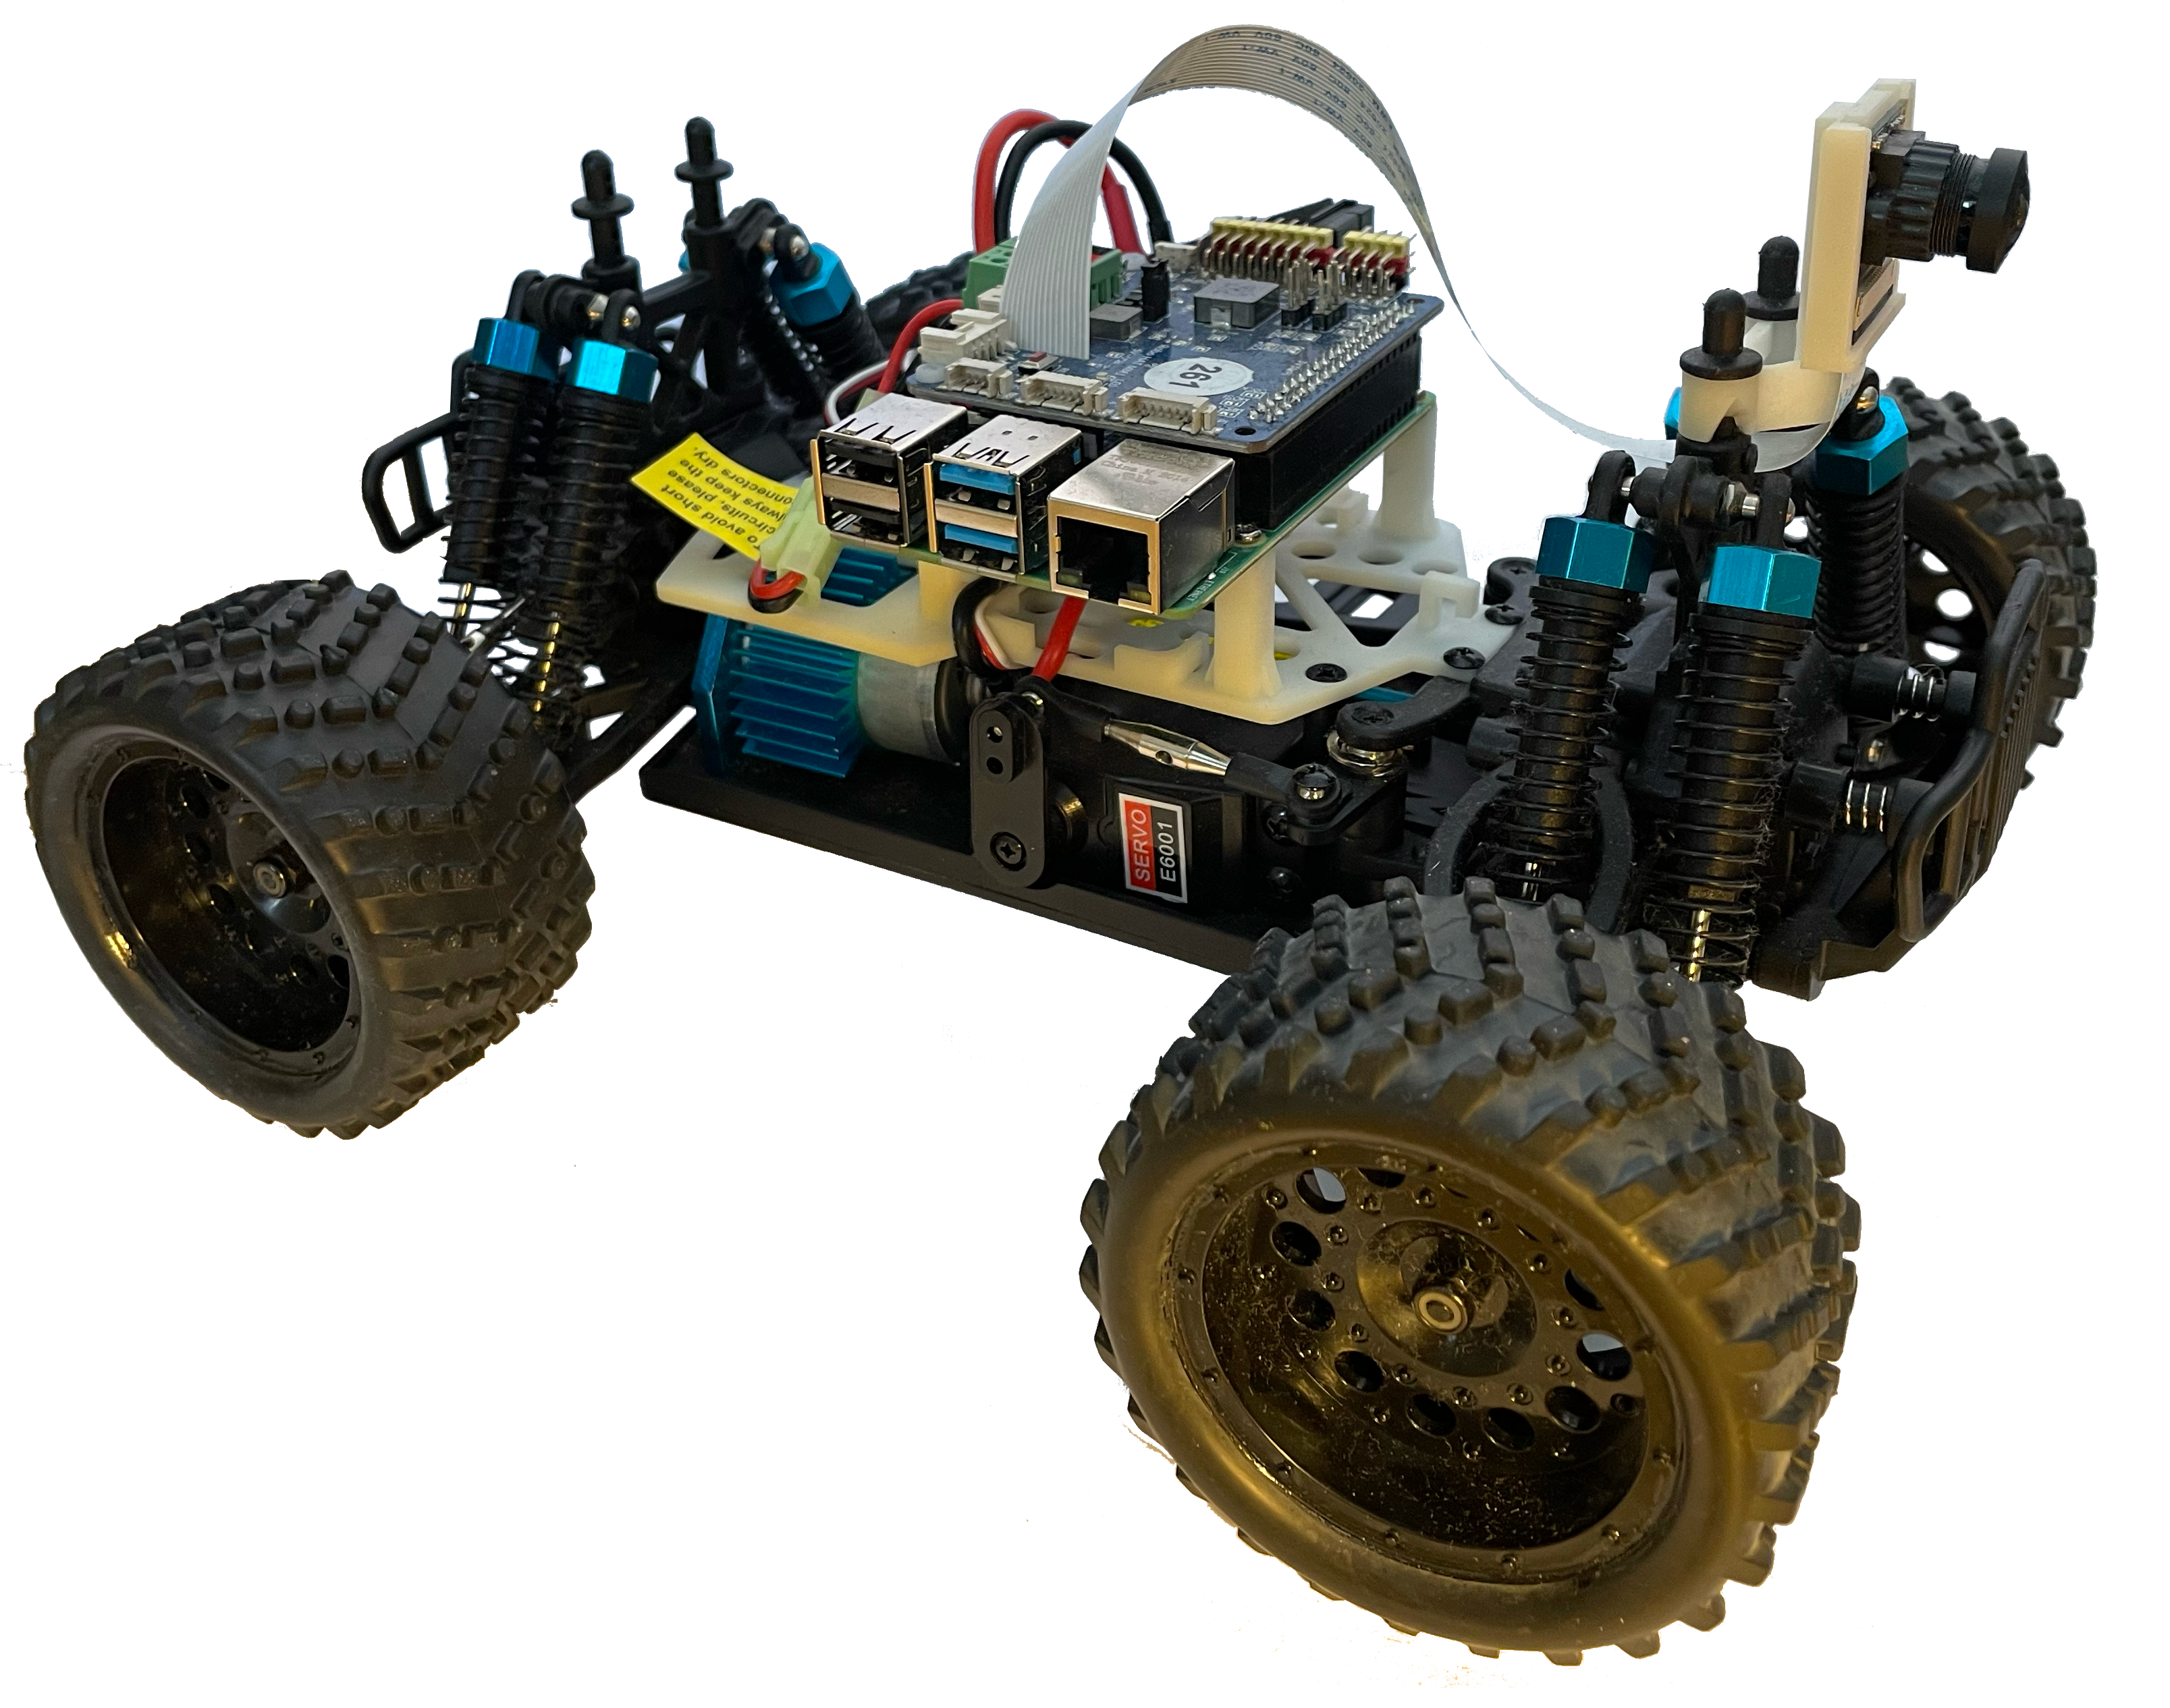
\includegraphics[width=0.6\textwidth]{figures/car_cut.png}
\caption{ Donkeycar S1 platform was used in the experiment. It comes equipped with a frontal camera, the only sensor used in the experiment. The sensor hat attached to the Pi micro-controller provides an IMU (Inertial Measurement Unit) sensor, not considered in the scope of the experiment.}
\label{fig:donkeycar}
\end{center}
\end{figure}

Donkeycar has an active community of machine learning and autonomous driving enthusiasts who keep improving the library and adding new features. Some improvements include traffic-light and stop sign detection using the external hardware Coral to process a benchmark object detection algorithm \parencite{coral}. This will not be used in this project as the focus of the research is the improvement of the neural network that predicts the vehicle's navigation. 

Another hardware that comes included with the car is the Inertial Measurement Unit (IMU) which is a set of inertial sensors attached to the Raspberry Pi that uses gyroscopes and accelerometers to track the movement of the device \parencite{Santiago}. It is possible to use the IMU information for navigation purposes. However, as this study aims to improve the generalization skills to unseen lighting conditions,  the only sensor used in this research is the one front camera attached to the vehicle.

The Donkeycar software was built upon open-source deep learning libraries such as OpenCV \parencite{opencv} for image processing, and Keras \parencite{keras} for training and running neural networks. Keras is a lightweight Python neural network library that runs on TensorFlow \parencite{tensor}, which the Donkeycar libraries use to train and run an autopilot neural network. From creating to driving autopilot networks, Donkeycar offers a variety of tools that allow fast experimentation. As shown in Figure~\ref{fig:cloning}, building neural networks with Donkeycar involves three steps a) to collect data using the car, b) to transfer the data to a host computer for cleaning and training the network, and c) loading the autopilot CNN on the Raspberry Pi in the scaled car and evaluating on a real-world setup.

\begin{figure} [!ht] %try to place the figure here (next option top of the page) 
\begin{center}
\includegraphics[width=1.0\textwidth]{figures/behaviorcloning.png}
\caption{ Donkeycar provides tools to collect and label expert demonstrations, clean inaccurate records from the dataset, and train deep neural networks.}
\label{fig:cloning}
\end{center}
\end{figure}

The Donkeycar autopilot machine learning networks are created using a form of supervised learning called behavioral cloning. The behavior of an expert is recorded and associated with labeled data and then used to train the network. The created CNN consists of an array of decision-making algorithms.

\subsubsection{Training Neural Networks}

Training a neural network involves providing examples of labeled data as input and applying mathematical and statistical concepts such as feed-forward and error backpropagation. Those functions will gradually reduce the error between the predicted output and the desired output across several iterations over the dataset \parencite{chang2018}. Each cycle of complete training iterations is called an epoch. The training session is composed of as many epochs needed until the network can no longer improve its prediction performance. 

Behind the curtains, a k-NN (k-nearest neighbors) algorithm trains a neural network. It accepts a set of training data and calculates the learning patterns of the data, computing the distance between the pixels in an n-dimensional space. It works similarly to a ranking algorithm in which the smaller distances are voted to the highest ranks.

The Donkeycar libraries facilitate this process, and the neural networks are trained using Keras. There are a few different built-in architectures available, and Keras linear is the standard neural network. According to the Donkeycar documentation, neural networks trained with linear architecture are robust and enable smooth steering. It also performs in low compute environments such as the Raspberry Pi 4 \parencite{donkeykeras}. This thesis trains the CNNs using the Keras linear neural network. It consists of a single output linear convolutional neural network composed of five convolution layers followed by two dense layers before the output of two dense layers with one output, each with linear activation for throttle and steering. 

The Donkeycar libraries enable the creation of well-performing networks using a relatively modest amount of data, which means that good CNNs can be created using five to ten thousand labeled images. However, such networks seem to overfit the conditions exposed during data collection, including lighting conditions. For instance, a network created with data collected during the daytime is unlike to perform well during night-time. In other words, the lighting levels seem to affect the network's performance considerably. 

Ideally, to create a robust CNN skilled enough to generalize well to lighting changes, the network would use samples of multiple lighting conditions. However, recording large amounts of data in different circumstances is not always feasible. Alternative training methods that help networks perform in unseen lighting conditions must be investigated. 

This research project explores the use of an adversarial defense training method to improve the capacity of deep learning neural networks to generalize to real-world changing lighting conditions. Different strategies to improve the neural network robustness, including image augmentation techniques such as image cropping, are commonly used and available in the Donkeycar platform. However, such methods are not investigated in this research as the focus is solely to measure the impact of adversarial defense training in the overall performance of the networks.

\subsection{Adversarial Machine Learning Attacks}

Adversarial machine learning attacks consist of methods to generate adversarial examples purposely designed to cause machine learning networks to fail in their predictions. However, despite causing great harm, the perturbations generated by the adversarial images can be subtle enough to be imperceptible to the human eye.

Adversarial attacks are organized into evasion, poisoning, and extraction attacks. However, evasion attacks are more likely to compromise safety because it can be carried out on a ADS while it is running. Such attacks can be white-box and black-box attacks. While the white-box attacks require having full access to the architecture and parameters of the network, the black-box attacks do not require knowing the network structure and architecture \parencite{piazzesi}. 
 
Adversarial examples have been widely used to fool neural networks successfully. However, the impact of adversarial images on the neural network's ability to generalize to real-world changing lighting conditions lacks a clear understanding.

\subsubsection{Adversarial Defense Training Method} 

It has been demonstrated the possibility to improve CNN's ability to generalize to unseen conditions and defend against adversarial attacks using adversarial images during the training process. The concept consists in modifying the standard training procedures and adding artificially generated adversarial images. Training CNNs additionally mixing standard and adversarial images have improved the network's robustness against adversarial images in simulation environments \parencite{Rosebrock}. 

In Figure~\ref{fig:adv} the adversarial training process is shown. Adversarial images are mixed with standard images to compose the set of data used by Keras to train the neural network.

\begin{figure} [!ht] %try to place the figure here (next option top of the page) 
\begin{center}
\includegraphics[width=0.9\textwidth]{figures/advtraining.png}
\caption{ The adversarial defense training method involves generating a batch of adversarial images and combining them as a single batch used for training the network \parencite{Rosebrock}.}
\label{fig:adv}
\end{center}
\end{figure}

To generate a total of N adversarial images, a network must be combined with the adversarial attack Fast Gradient Sign Method (FGSM). The FGSM is a reliable way to generate adversarial examples that cause neural networks to misclassify their input \parencite{Goodfellow}.

See in Figure~\ref{fig:fgsmpanda} how a discrete perturbation could be added to the input causing the neural network to fail the classification task.

\begin{figure} [!ht] %try to place the figure here (next option top of the page) 
\begin{center}
\includegraphics[width=0.8\textwidth]{figures/goodfellow-fgsm.png}
\caption{ On the left-hand side of the image, a CNN is used to correctly classify a panda picture in the class "panda" with 57.7\% of confidence. In the middle, a gradient descent noise vector is constructed using "0.007" as the epsilon value that defines the norm of the perturbation, which is itself erroneously classified as a type of worm called a nematode. The noise vector is added to the original image, resulting in the same CNN misclassifying the panda as an ape species called gibbon with 99.3\% confidence. Image source: Explaining and Harnessing Adversarial Examples \parencite{Goodfellow}.}
\label{fig:fgsmpanda}
\end{center}
\end{figure}
The FGSM is a fast and straightforward method to construct adversarial examples. The technique adds perturbations and linearizes the cost function in the gradient direction. As shown in the Equation ~\ref{equ:grad}, a function which specifies that the adversarial image results from the sum of the image \(X \)with the sign function, which takes as the input parameters the accurate label of \(X\). \(J\) is the cost function that was used to train the network, and \(X J()\) represents the gradient of \(X\) and the epsilon factor. Finally, \(Xadv\) is the resulted adversarial image from the original image \(X\)
 \parencite{changli}.
 \begin{center}
\begin{equation}
Xadv = X + sign(X J(X, y))
\label{equ:grad}
\end{equation}
\end{center}

The FGSM advantages include low computational complexity and high transfer rate, making them appropriate for low processing power computers such as the Raspberry Pi. On the other hand, some disadvantages of the FGSM are a low attack success rate, and perturbations are applied on a single image. In contrast, there are universal image-agnostic perturbation attacks methods that fool classifiers by single adversarial perturbation to all images \parencite{changli}.

Using gradient techniques differs from other image augmentation forms, such as brightness or blurring techniques. The directional change in image intensity defines the gradient, which represents the image comparison of front and background in edge detection recognizing areas of high or lower contrast \parencite{gradient}. At each input image pixel, a gradient measures the change in pixel intensity in a given direction. Estimating the direction, orientation and the magnitude of the change in direction makes it possible to detect regions of an image that look like edges. 

Kernels are used to estimate gradients and find the structural components of the image. For gradient estimation, the first step is to find and mark the north, south, east, and west pixels surrounding the center pixel. The gradient magnitude measures how significant the change in image intensity is. A gradient magnitude is a real-valued number that quantifies the strength in intensity.
The gradient orientation determines the direction in which the change in intensity is pointing and provides an angle to quantify the direction of the change. Convolutions are then used to define the orientation and magnitude, computing the difference in the vertical and horizontal changes to determine the intensity and direction of pointing.

The FGSM is considered a white-box, gradient-based, non-targeted attack. Unlike black-box attacks, where the attacker has no access to the neural network infrastructure, white box attacks are situations when the attacker has access to the target network's parameters and architecture. As this study investigates the possibility of using adversarial defense training methods to improve the performance of the self-driving CNN, enabling generalization to external lighting conditions in a real-world setting, having access to the network is expected.

This thesis analyzes the impact of neural networks running in low processing power micro-controllers, so low computational complexity is crucial. The disadvantages of the method are not deterring as the low attack success rate does not out-weight the possible benefits of an improvement in a training process. Therefore, FGSM is the adversarial machine learning method chosen to improve the networks' performance in unseen lighting conditions. 

\subsubsection{Safety and Performance}

Researchers measured the impact of adversarial attacks on the driving safety of vision-based ADS by constructing an end-to-end evaluation framework with a set of driving safety performance measures. The collision rate and the success of route completion rate were some of the criteria used to validate the results under the perturbation attack \parencite{zhang}.

In another research, the impact of adversarial attacks on the performance of self-driving CNNs was measured by analyzing how autonomous driving CNN's deployed in a simulation environment react to several different adversarial attacks. By analyzing the rate of collisions in various circuits in a specific set of pre-defined conditions, it was shown that the adversarial attacks significantly impacted the driving neural networks, leading to collisions in all four evaluations during inference time \parencite{piazzesi}.

A study compared the performance of different self-driving convolutional neural networks in the same circuit using standard training techniques. The manual recovery from collisions, also known as human interventions, together with the lap time, were used as a measure of success. In the study, the author demonstrated that the best-performing CNN could drive five laps without human intervention, revealing the capability of end-to-end neural networks as a feasible option for autonomous driving research \parencite{liivak}.

The number of collisions accounted in \(N\) elapsed circuit has been used successfully to demonstrate the capabilities of self-driving networks. In this study, walls were built surrounding the track lane, and crashes against the wall were measured and compared to evaluate the performance of different neural networks. 

\newpage
\section{Method}

This section describes the plan and the procedures to use adversarial defense training methods to train a CNN supervised classifier autopilot using behavioral cloning with a 1:10 scale car based on the open-source platform Donkeycar.

The project aims to train neural networks to autonomously drive a car and then improve their generalization ability to never-seen-before lighting conditions. The method is divided into two high-level blocks, developing the CNNs and evaluating the networks. The development stage includes data collection and labeling during expert demonstrations and training of the CNNs using the built-in Donkeycar neural network. The final step involves evaluating the CNN's self-driving abilities in the circuit.

The research project was formatted in a factorial design, with multiple independent variables being manipulated (Table~\ref{tab:datacol}). The summary of the main stages and how the independent variables of the experiment affect the dependent variable are specified in Table~\ref{tab:indvar}.

\begin{table}[H]
\begin{center}
\begin{tabular}{  |p{8cm}|p{4cm}| } 
\hline
 \multicolumn{2}{|c|}{\textbf{Data collection and labeling}} \\
\hline
\textbf{Independent variables} & \textbf{Values} \\
\hline
Light & low  \\ 
Laps & 20 and 40 \\ 
Images & 20 per second \\ 
Label 1 (throttle) & [0, 1]\\ 
Label 2 (steering angle) & [-1, 1] \\ 
Two datasets & small and large\\ 
\hline
 \multicolumn{2}{|c|}{\textbf{Training the CNNs}} \\
\hline
\textbf{Independent variables} & \textbf{Values} \\
\hline
Dataset & small and large \\ 
Image data augmented by adversarial attack data & no, yes \\ 

\hline
\end{tabular}
\caption{\label{tab:datacol}The study's independent variables were manipulated to measure the results of the dependent variable, which is the number of collisions during a two-laps performance. The throttle value ranges from 0 when stopped to 1 at full speed. The steering system has a steering angle of -1 when at -30 degrees left turn and 1 at +30 degrees right turn. The low lighting levels mean a darker room, where the intensity of the room lights applied during data collection is considerably lower than the unseen higher levels, which were used to evaluate the network generalization skills. 
}
\end{center}
\end{table}

Initially, data is collected using a frontal RGB camera attached to the scaled vehicle. At the same time, the expert drives along the circuit using a joystick, the behavior of the expert is recorded in the form of a batch of images captured at a rate of 20 images per second, and each image contains a corresponding steering angle, throttle and timestamp labels. Despite the expert's best effort, collisions or near misses are inevitable. Thus, the data must be cleaned, and inaccurate records are removed from the recordset before being used in the next phase, training the neural network. 

In the next stage, the cleaned data, which includes a batch of labeled images, is used to train a Donkeycar built-in convolutional neural network architecture with imitation learning, as described in section 2.3.2. Finally, the newly created self-driving CNNs are evaluated in four distinct conditions. 

\begin{table}[H]
\begin{center}
\begin{tabular}{  |p{8cm}|p{4cm}| } 

\hline
\multicolumn{2}{|c|}{\textbf{Evaluating the CNNs}} \\
\hline
\textbf{Independent variable} & \textbf{Values} \\
\hline
Laps & 2 \\ 
Lights & low, high \\ 
Vision & uncorrupted, corrupted \\ 
\hline
\textbf{Dependent variables} & \textbf{Values} \\
\hline
Collisions & [0...n] \\ 
\hline
\end{tabular}
\caption{\label{tab:indvar}The neural networks' performance is evaluated during the inference time. The collisions are measured while performing two laps in the circuit under four different conditions, including darker and brighter lighting levels and the addition of adversarial corrupted vision perturbations to all input images during inference time.
}
\end{center}
\end{table}

The first and second conditions will evaluate the performance of the trained CNNs when it is exposed to the same lighting conditions used during the training phase. The third and final conditions will evaluate the CNN while exposed to unseen higher lighting conditions. The results of the first evaluation phase will establish the baseline. Depending on the results, if the network fails to generalize to unseen lighting conditions, then an adversarial defense training method will be employed to improve the CNN generalization skills. 

During inference time, some conditions include submitting the neural networks to classify a corrupted vision created by generating adversarial attacks like modifications of the real-time image on the fly. It is important to note that every image exposed to the CNN for classification is corrupted when using adversarial attacks.

One control condition was selected for internal validity compared with the other experimental conditions. The control condition is defined using a smaller dataset (M-TS) when evaluating the CNN. Performance measurements are collected after exposing the CNN to lower lighting levels, using a standard training method described in 2.3.1, and are performed without direct adversarial attacks. 

The CNNs' performance is collected in the evaluation stage and then compared against the baseline to evaluate and measure success. Details of all the experiment stages are described in the following subsections.

\subsection{Experimental Setup}

To train an autopilot with Keras, the Donkeycar recommends collecting five thousand images as the minimal amount to produce a neural network that performs acceptably in a given circuit \parencite{donkey-keras}.  
To collect the data necessary for the experiment, the front-facing wide-angle camera in the vehicle captures the images. At the same time, Donkeycar scripts automatically label them with steering angle and throttle values. Two sets of data were collected in two different sessions, the first containing approximately five thousand images and a second larger dataset containing about ten thousand images. The need for two datasets with different sizes is to compare the results and evaluate the impact of the volume of data on CNN's overall performance in two distinct scenarios. 

\subsubsection{Description of the Evaluation Conditions}

The experimental results are based on the platform's performance described in the previous subsection. Five points cover a range of locations in the track to illustrate different lighting conditions. The points consist of areas captured by the platform that drives in the circuit until it cannot proceed due to a collision with the wall. In all conditions, the shape of the circuit remains unchanged. However, the light intensity is modified. 

The CNNs are trained only with the data captured in the first condition in lower lights. Thus, the CNNs will have their generalizations skills evaluated in unseen lighting conditions when exposed to higher-light conditions. The vehicle's camera captures twenty frames per second. The dataset is stored, cleaned, and used in successive training.

An expert policy is collected in two different sessions. The first session performs 20 laps, and the second session collects 40 laps, gathering approximately 5000 images and 10000 images, respectively. All images are labeled with their corresponding steering angles and throttling values.
The steering has number values within the range of [-1.0, 1.0], in which negative values correspond to turning to the left, and positive values correspond to turning to the right. Throttle values are within [-1.0, 1.0], in which zero the vehicle is stopped. Positive values mean forward-moving, while negative values mean backward moving. One caveat is that only forward moving is considered in this study. Thus, human intervention was necessary to recover the car from collisions and recenter it in the lane.  

Four different autopilot neural networks are created. The first network is trained with a smaller dataset. The second network uses the same data as the first network but is created using an adversarial defense training method. The third network is trained with a larger dataset, and the final network uses the same data as the third network. Still, it is created using the same adversarial defense training method used in the second network. 

Defense methods improve the expert policy's generalization skills to unseen lighting conditions. Therefore, all four networks are evaluated while exposed to four different conditions. In the first condition, the autopilot CNNs are evaluated in lower lights, with the same level of illuminance captured during the data collection phase. The second condition involves using the same lower-light environment to run the CNN while under the same adversarial attack used for the defense training method. The CNN is evaluated in an unseen higher-lighting environment in the third condition. In the final condition, the CNN's are evaluated in the same previous unseen higher-lighting environment but under the adversarial attack. 

An adversarial image generator must be integrated with the platform to evaluate the different networks under established conditions. Specific implementation settings and values will differ depending on the experiment environment. This step includes performing iterations to find appropriate values. 

Once the driving platform is implemented and integrated with the adversarial defense training methods, a measure must be provided to allow comparison. The measurement should quantify the autopilot CNN's performance and the circuit's lower and higher lighting conditions. 

The final purpose is to create a proof of concept strategy for training more skillful CNNs capable of generalization to unseen lighting conditions. 

\subsubsection{ADS Platform}

The testbed architecture is designed for training and evaluating behavior cloning neural networks on car-like robots, such as the Donkeycar. The scaled vehicle is equipped with a mono frontal wide-angle RGB camera, capturing 120x160  images labeled with the motor throttling and steering angle values used to classify, create, and evaluate a self-driving neural network. 

A Raspberry Pi 4 microcontroller is used to run the Keras deep learning libraries using a TensorFlow backend to trigger commands to servo-controlled steering and thrust motors. The CNN is trained on an indoor circuit constructed with white gaffer tape and cardboard walls. Although the Donkeycar design allows for the integration of sensors such as LiDAR and IMU, such sensors will be kept out of the project's scope, as the object of analysis is solely the input of the RGB camera system instead.

\subsection{CNN Model Training}

Training a convolutional neural network consists of pairing the images captured by the camera with corresponding labels with throttle and steering angle values, which will then be used to train a CNN capable of steering a car in a circuit. The approach taken to train the CNN is behavioral cloning, a form of supervised learning in which labeled data is created by recording the behavior of an expert. A combination of open-source projects is used to create neural networks. The Keras and TensorFlow libraries convert the images to arrays of vectors, also called tensors, which allow to load input images using OpenCV and represent them as a Numpy array of numbers. In this way, they can be converted back to a format compatible with Keras and TensorFlow that represents images as tensors containing the image high, width, and channels.

Deep learning is applied for training a convolutional neural network on the image dataset, which consists of the circuit and its surroundings or everything that was captured by the camera attached to the car. The training and validation are performed using a split of the dataset with a ratio of 0.8:0.2, and the validation occurs during a set of iterations called epochs. The goal is to train the CNN to identify a class a given image belongs to.

After the neural network architecture of the autopilot has been successfully trained, it classifies the input image and predicts the most suitable throttling value and steering angle. The CNN architecture used in this project was the default Donkeycar linear network, consisting of five convolution layers, a flattening layer, and three fully-connected layers.

\subsubsection{Standard CNN Training Method }

The standard behavior cloning training approach to creating a CNN capable of steering a car in a circuit presenting a behavior similar to an expert is a straightforward process. It includes first capturing images using the open-source project OpenCV as part of the vehicle and then storing them on a path containing a JSON file comprising the class "ground truth" labels. The images are captured in a range of 20 images per second. As demonstrated in  Figure~\ref{fig:standardtraining}, in the standard training procedure, a sample portion of the dataset is selected for training. Donkeycar uses Keras to randomly select 80\% of the images as the training set and 20\% as the validation set.

\begin{figure} [H] %try to place the figure here (next option top of the page) 
\begin{center}
\includegraphics[width=0.5\textwidth]{figures/standard-training.png}
\caption{ The normal process of training is described in which N images are sampled from a dataset to train a CNN \parencite{Rosebrock}.}
\label{fig:standardtraining}
\end{center}
\end{figure}

The final stage of the standard process of training CNNs includes using a fit function that takes the training set and the validation set as parameters. The convolutional network uses Keras and TensorFlow image processing filters chained together to implement 2D convolutions,  dropout, and classifiers functions such as dense and activation.
 
This approach limits the CNN to perform well only under the circumstances presented in the dataset. The CNN usually fails in unseen conditions, such as different lighting conditions. As a result, a CNN performs well in conditions similar to the original dataset but poorly in other lighting conditions. A different approach using a mix of adversarial images and regular images could be used to augment the dataset and improve the CNN generalization skills.

\subsubsection{Adversarial Defense Training Method}

The adversarial training defense method to train deep neural networks includes mixing adversarial images to the dataset to improve the robustness of the CNN and its generalization skills \parencite{Rosebrock}. The process is similar to the previous standard method but slightly more sophisticated. As illustrated in Figure~\ref{fig:advdefensemethod}, the adversarial defense method includes combining the original images and synthetically generated adversarial images into a single dataset used to train the CNN.

\begin{figure} [H] %try to place the figure here (next option top of the page) 
\begin{center}
\includegraphics[width=0.8\textwidth]{figures/advtraining.png}
\caption{Illustration of the adversarial defense training method which mixes normal images and adversarial images when training CNNs \parencite{Rosebrock}.}
\label{fig:advdefensemethod}
\end{center}
\end{figure}

The training pipeline itself is not changed compared to the standard training procedure, in which convolutional neural network architecture is trained on sample images of a dataset. However, the dataset comprises an equal split of standard images and a batch of generated adversarial images constructed using the Fast Gradient Sign Method attack and the CNN itself. 

Although adversarial images usually aspire to a negative connotation, primarily because of the vulnerability of deep learning networks, adversarial images can theoretically be used as an advantage to construct CNNs capable of generalizing better to unseen conditions. Thus, the working horse of this approach is the function to generate batches of adversarial images that could be used to create more robust CNNs. 

\subsubsection{Adversarial Images Batch Generator}

The adversarial defense training method is defined as the idea that the original dataset of examples can be augmented before training the network without spending extra time collecting data with an expert. This technique uses the FGSM function, as shown in Figure~\ref{fig:advpattern} to generate an adversarial pattern that can be added to the image. The function inputs the CNN, which was previously constructed with the original dataset, a sample image, and the labels, to return a perturbation vector.

\begin{figure} [H] %try to place the figure here (next option top of the page) 
\begin{center}
\includegraphics[width=0.8\textwidth]{figures/adversarial-pattern.png}
\caption{ The function to generate an adversarial pattern takes an instantiation of the CNN architecture, trained on the original dataset, the image to be perturbed, and the labels \parencite{Rosebrock}. }
\label{fig:advpattern}
\end{center}
\end{figure}

The function to generate the adversarial pattern first cast the input image to a float 32-bit data type. Then monitor gradience by watching the image and using the CNN to make predictions on the image, computing the loss concerning the original class label, and passing the label and the prediction producing the results from the means square loss function (MSE) and returning a loss value. Finally, it calculates the gradience using the loss and the image to output the sign gradient that is returned by the function.

The function to generate the adversarial perturbation is only part of adversarial defense training. Next, it is necessary to create another function to generate a set of image adversaries to be used to fine-tune the CNN. The adversarial images and the standard images are mixed and added to the training pipeline. As demonstrated in Figure~\ref{fig:batchadv} the process of creating a batch of adversarial images consists of iterating through each image available in a Donkeycar tub, which is a folder containing the images and labels generated by the expert, and making a perturbed copy of the image in a new tub.

\begin{figure} [H] %try to place the figure here (next option top of the page) 
\begin{center}
\includegraphics[width=0.8\textwidth]{figures/batch-adversarial.png}
\caption{ To generate a batch of adversarial images, a copy of each original image is created, preserving the original "ground truth" labels but modifying the image with an additional perturbation \parencite{Rosebrock}.}
\label{fig:batchadv}
\end{center}
\end{figure}

The perturbation is used to construct the adversarial image by taking the signed grad and multiplying it by the epsilon factor, and the gradient update is added to the image. It converts the image to a Numpy array from the TensorFlow volume and returns an image adversary. Higher is the epsilon factor, also higher are the chances of the manipulation being able to be perceived by the human eye. Notice that it keeps the correct label despite adding perturbations to the image. See in Figure~\ref{fig:attackstandard} the comparison of the standard image with an image that has been generated using the adversarial perturbation.

\begin{figure} [H] %try to place the figure here (next option top of the page) 
\begin{center}
\includegraphics[width=0.8\textwidth]{figures/attaked-standard-images.png}
\caption{On the left is a standard image that was captured in lower-light conditions. The same image has been duplicated on the right, applying the FGSM perturbation's addition with an epsilon factor of 0.8.}
\label{fig:attackstandard}
\end{center}
\end{figure}

The function receives an instance of the CNN, which was generated previously, a base input image and the delta, which is the noise vector used for constructing the adversarial image and the label. The perturbation is added to the base image with the delta vector and will clip all the pixel values to the range from 0 to 255 and converts the image from a floating-point data type to an unsigned 8-bit integer. 

A batch of the same size as the original dataset is generated at the end. It is composed of adversarial images, which are then mixed with the original dataset. The training images will be sampled randomly from standard and adversarial examples. 

Limitations to this method include the fact that depending on the CNN and the optimizer, generating a robust neural network that can generalize better to adversarial conditions and have a more accurate driving might be necessary to fine-tune the CNN using different epsilon factors. 

The goal is to solve the problem of the CNN being overfitting to the trained conditions. When overfitting, the network is close to memorizing the training set and fails to generalize to unseen images. Techniques including data augmentations to validation and training set splits might reduce the impact of overfitting.

The neural network architecture used to train the CNNs in this project was the default Donkeycar linear architecture, consisting of five convolution layers, a flattening layer, and three fully-connected layers. The performance of all networks is recorded and evaluated regarding their accuracy in maintaining steering clear of collisions. Accurate networks should classify the input image and predict the most suitable throttling value and steering angle. 

\subsection{Design and Implementation of the Evaluation}

The experiments were performed on the autonomous car under sixteen different conditions to evaluate the performance of four distinct networks. The goal is to answer the research question by demonstrating the impact of (a) lighting conditions, (b) the size of the data set, and (c) adversarial training methods on the performance of the driving algorithms in a scaled real-world setup.

The four conditions in which the CNNs are evaluated are the following:


\begin{itemize}

   \item L - Lower lighting levels refer to a condition in which the room has darker lighting intensity with an average lux of 19.6.
   
    \item H - The room lighting intensity is brighter with an average lux level of 81.2. 
   
    \item LC - The same lower-level lights are applied in this condition. However, the vision is corrupted with adversarial images replacing the standard input images during inference time.
   
   \item HC - Adversarial corrupted images again replace the standard input images at inference time while brighter lighting levels illuminate the room.
\end{itemize}

\subsubsection{Evaluating M-TS}

Each evaluation stage creates a different CNN, which is evaluated under four distinct conditions. The first CNN to be evaluated was trained with a smaller dataset consisting of images collected during 20 laps, which is first deployed for evaluation in the same lighting conditions exposed during training. The measure values established in this first condition will define the baseline. The baseline measure will be used as the criteria to evaluate if the process is successful or not. In addition, to attain success, the network would need to improve its performance concerning the baseline. A CNN should perform at least two laps without collisions or human interventions if well trained. 

\begin{table}[h]
\begin{center}
\begin{tabular}{ |p{3cm}|p{1cm}|p{2cm}|p{1cm}|p{1cm}|p{1cm}|p{1cm}|  }
 \hline
 \multicolumn{7}{|c|}{Evaluation conditions} \\
 \hline
 CNN Model & Laps & Images & L & LC & H & HC \\
 \hline
M-TS & 20 & \textasciitilde5000 & 19.6 & 19.6  & 81.2 & 81.2\\
\hline
\end{tabular}
\caption{\label{tab:cond1method}The CNN was evaluated in four different conditions. The M-TS CNN was generated using the sample data collected over 20 laps of expert demonstration in a total of approximately 5000 images (20 images per second). The four conditions evaluated include lower lighting (L), lower lighting under adversarial attack (LC), higher lighting levels (H), and higher lighting with the adversarial attack (HC). The average luminance in lower lighting is 19.6 lux, whereas the average luminance rises to 81.2 lux in higher lighting.  }
\end{center}
\end{table}

As shown in Table~\ref{tab:cond1method}, the CNN is evaluated under an adversarial attack during inference time. The resulting measure will be compared against the baseline. For the adversarial attack to be considered successful, the CNN performance deteriorates compared to the baseline. It is expected that the network would misbehave when exposed to adversarial images.

The next stage includes evaluating the CNN in unseen conditions. The circuit is exposed to higher levels of light intensity. CNN's behavior is unknown. However, it might become unstable. Hence, the need for mechanisms that safeguard against such adversities.

Finally, the CNN is evaluated in the last condition, in which the same higher levels of light exposure are maintained from condition three. However, an additional adversarial attack is also used against the network, which is expected to misbehave if the adversarial attacks succeed. 

This step aims to identify whether the performance of a self-driving CNN is affected by unseen lighting levels or a selected adversarial attack.

\subsubsection{Evaluating M-TSA}

The second CNN (M-TSA) evaluated in the experiment consists of a mix of the standard records used to train the first CNN M-TS and adversarial images. This time an adversarial training method is used instead of the standard training method used in the previous network. The intention is to create an improved CNN that outperforms the standard network in generalizing unseen lighting conditions and is resilient against the adversarial attack.

As shown in Table~\ref{tab:test3method} the dataset has increased in size while keeping the same number of laps. This occurred because the extra added images were artificially generated using the Fast Gradient Sign Method mentioned previously.

\begin{table}[h]
\begin{center}
\begin{tabular}{ |p{3cm}|p{1cm}|p{2cm}|p{1cm}|p{1cm}|p{1cm}|p{1cm}|  }
 \hline
 \multicolumn{7}{|c|}{Evaluation conditions} \\
 \hline
 CNN & Laps & Images & L  & LC  & H  & HC \\
 \hline
 M-TSA & 20 & \textasciitilde10000 & 19.6  & 19.6  & 81.2 & 81.2\\
\hline
\end{tabular}
\caption{\label{tab:test3method}The CNN M-TSA was evaluated in the same conditions as the previous networks. However, this CNN was created by using an adversarial defense training method in which an additional batch of adversarial images is included in the training sample dataset.}
\end{center}
\end{table}

Similar to the previous stage, the new CNN is evaluated in four different conditions. The first is the standard condition, which means the same lighting conditions that the CNN was trained with. The second condition involves deploying an adversarial attack against the CNN while performing in the circuit during inference time, maintaining the standard low light levels used during training. 

In the third condition, the CNN is performed under exposure to unseen higher lighting conditions. This stage verifies if the proof of concept defensive training method improves the CNN's generalization to unseen lighting levels. 

Additionally, the final condition of this evaluation stage maintains the higher lighting levels of the previous condition to evaluate the CNN's performance trained with an adversarial defense method against the same adversarial attack that it has been trained with while exposed to unseen lighting intensity. 

\subsubsection{Evaluating M-TL}

The third evaluation stage involves creating a new CNN trained with a larger dataset consisting of images collected during 40 laps, twice as much as the previous CNN models. The goal is to understand if the addition of more data alone would be sufficient to create a more skilled CNN capable of generalization to unseen lighting levels. 

As shown in Table~\ref{tab:test2method}, while maintaining a standard training method, the lighting levels in each condition are the same for evaluating all networks. The difference is within the CNN considered, which uses a more extensive dataset. 

\begin{table}[h]
\begin{center}
\begin{tabular}{ |p{3cm}|p{1cm}|p{2cm}|p{1cm}|p{1cm}|p{1cm}|p{1cm}|  }
 \hline
 \multicolumn{7}{|c|}{Evaluation conditions} \\
 \hline
 CNN & Laps & Images & L & LC & H & HC \\
 \hline
 M-TL & 40 & \textasciitilde10000 & 19.6 & 19.6 & 81.2 & 81.2\\
\hline
\end{tabular}
\caption{\label{tab:test2method} The CNN model M-TL was trained with the same standard training procedure used in the first CNN, but additional laps were added to the training sample. The average luminance levels are the same as in the previous evaluation stage. }
\end{center}
\end{table}

The network is first deployed for evaluation in the same lighting conditions exposed during training. If well trained, using only standard approaches, the M-TL network should perform at least two laps without collisions or human interventions. 

The second condition involves deploying the adversarial attack against the CNN trained with the larger dataset, initially maintaining the lighting levels. For the third condition of this evaluation stage, the CNN is exposed to unseen higher lighting levels. Moreover, the higher lighting levels are maintained for the final condition, and an additional adversarial attack is deployed against the CNN during inference time while it is performing in the circuit.

This step aims to identify whether the performance of a self-driving CNN is affected by the amount of data when using a standard training method.

\subsubsection{Evaluating M-TLA }

The final evaluated CNN (M-TLA) uses the same larger dataset used in M-TL. However, it is trained with adversarial defense methods instead. The goal is to identify the impact of creating networks trained with adversarial defense methods using a larger dataset.

As shown in Table~\ref{tab:test4method} the CNN evaluated in this stage is created from the most extensive dataset used in the experiment, containing approximately 20000 images in total, including adversarial images artificially generated. The average lighting conditions remained the same as in the previous evaluation stages. 

\begin{table}[H]
\begin{center}
\begin{tabular}{ |p{3cm}|p{1cm}|p{2cm}|p{1cm}|p{1cm}|p{1cm}|p{1cm}|  }
 \hline
 \multicolumn{7}{|c|}{Evaluation conditions} \\
 \hline
 CNN & Laps & Images & L  & LC & H  & HC \\
 \hline
 M-TLA & 40 & \textasciitilde20000 & 19.6 & 19.6  & 81.2 & 81.2\\
\hline
\end{tabular}
\caption{\label{tab:test4method}The final CNN was created using the most extensive dataset. The sample training data contains examples of driving behavior for 40 laps. Additionally to the standard samples, adversarial images were added to the training batch. The lighting levels were consistent across all evaluation stages for each evaluation condition. }
\end{center}
\end{table}

The same four conditions applied in the previous evaluation stage are also applied when evaluating the CNN model M-TLA. Initially, the network is evaluated in the same conditions that were used to collect the data, including lower lighting conditions. The following condition involves preserving the lower lighting levels and analyzing CNN's performance under attack by adversarial images. 

The CNN is exposed to unseen higher lighting levels for the last two conditions. An adversarial attack is also generated against the network to evaluate it under the fourth and last condition. 
This phase aims to understand if the CNN's performance is affected by using a larger dataset for generating networks using adversarial training methods.

\subsubsection{Evaluation Measure}

The CNN's performance in the circumstances exposed during the training will define the baseline measure. Standard training techniques should create a network that runs precise maneuvers collision-free in a circuit for at least two laps. It is unknown how the networks will perform in unseen lighting conditions, but we expect the driving to be correct under the same conditions the CNN was trained in, and collisions should be zero. Thus, the number of crashes that occurred when running the car for two laps in the circuit is the quality yardstick used to measure the performance of the networks.

\clearpage %if newpage doesn't work
\section{Results}

As described in the method section, the study was divided into two main stages, creating and evaluating four deep neural network models created to answer the research question. The network development stage included the data collection and labeling, which recorded the behavior of an expert demonstration in the form of labeled images, and the use of the images for training neural networks using the built-in Donkeycar CNN architecture, and two different datasets were used to train the CNNs, one smaller and one larger. The performance of a scaled car loaded with neural networks was evaluated in a real-world setup. Four different neural networks were created using two different training approaches, a standard training approach and an adversarial defense training method. 

The data collection process took place only under low light conditions. Four evaluations were performed to measure each neural network's performance in four conditions, including unseen higher lighting levels. This section analyzes the results of the experimental setup and training methods used in the process. Finally, the performance of the car in the circuit is measured, and the results of the evaluation in different conditions are divided into four main categories: 

\begin{itemize}

   \item Evaluating M-TS - measures the CNN's performance created with a smaller data set using standard training methods, which means only training the networks using image samples of lower-lighting exposure.
   
    \item Evaluating M-TSA - analyses the performance of the CNN model M-TSA created using the same smaller data set used in M-TS in addition to a batch of adversarial images, incorporating a slightly more complex adversarial training method.
   
   \item Evaluating M-TL - the same standard training process and lower light conditions are used to train the M-TL CNN. However, a larger data set is used for the training instead. 
   
   \item Evaluating M-TLA - the neural network CNN model M-TLA is created by implementing the adversarial training method using a mix of the larger dataset in addition to an equally large batch of adversarial images.
\end{itemize}
 
The aim is to demonstrate the navigation capabilities of the driving networks and their ability to generalize to unseen lighting conditions. To illustrate the consequences of adversarial attacks on CNN's performance and show how the adversarial defense training method improves generalization skills in a scaled real-world setup.

\subsection{Data Collection and Labelling}

The starting point for training a neural network to drive autonomously in a circuit using behavioral cloning is to generate a clear policy to teach the car how to behave when launched on the track. This process is called data collection, in which labeled images are recorded while an expert demonstrates how driving should be performed. The expert drove two sessions to collect data, one shorter session, and one more extended session. It is crucial to notice that both were completed in lower light sessions. Thus, each CNN could be evaluated when performing in unseen higher lights levels. The networks are also evaluated while being under attack in both lighting conditions. The summary of all assessed conditions during the experiment is displayed below.

\begin{table}[H]
\begin{center}
\begin{tabular}{ |c|c|c|c|c| } 
\hline
Conditions & L & LC & H & HC \\
\hline
Lighting Levels & Low & Low & High & High \\
Adversarial Attack & False & True  & False & True \\
\hline
\end{tabular}
\caption{\label{tab:conditions}The four networks evaluated in the experiment are exposed to four conditions: lower-lights (L), lower-lights under attack (LC), higher-lights (H), and higher-lights under attack (HC).}
\end{center}
\end{table}

The summary of all evaluated conditions is displayed in Table~\ref{tab:conditions}. All the data collected in this experiment was under the lower-light levels. Therefore, the baseline is defined, measuring the CNN's performance in this condition. To achieve consistency and precision over the lumminance levels and prevent contamination with natural light exposure, the data was collected indoors in a sealed laboratory room with a controlled artificial light source. As demonstrated in Figure~\ref{fig:light}, the luminance levels in five critical points in the circuit are measured under two distinct conditions.  

\begin{figure}[H]
\begin{center}
\includegraphics[width=0.8\textwidth]{figures/lights.png}
\caption{ The standard lower-light conditions used to collect the data set for training all networks are on the left. On the right, the circuit is exposed to higher-lights unseen to the CNN, and no data was collected under this condition. }
\label{fig:light}
\end{center}
\end{figure}

To measure lighting levels in the circuit, the light meter LM-3000 \parencite{lightmeteraccuracy} was chosen as an in-depth article comparing several light meters point to it as the one clear winner as the most accurate option \parencite{lightmeter}. As demonstrated in Table~\ref{tab:lightlevels}, different points of the circuit track had other light level measurements, with levels over four times higher in the brighter conditions.

\begin{table}[H]
\begin{center}
\begin{tabular}{ |c|c|c|c| } 
\hline
Position on the circuit & Lower-lights - L (lux) & Higher-lights - H (lux) \\
\hline
A & 21 & 110  \\ 
B & 19 & 86 \\ 
C & 19 & 75 \\ 
D & 19 & 75 \\ 
E & 20 & 60 \\ 
\hline
Average & 19.6 & 81.2\\
\hline
\end{tabular}
\caption{\label{tab:lightlevels}The four networks evaluated in the experiment are exposed to four conditions: lower-lights (L), lower-lights under attack (LC), higher-lights (H), and higher-lights under attack (HC).}
\end{center}
\end{table}

The four networks evaluated in this experiment were only trained using the images captured in lower-light conditions. However, two distinct training methods were applied to improve the CNN performance in the unseen higher-light conditions, a standard training method and one adversarial defense training method. 

The first step for training a self-driving neural network involves having an expert demonstrate a driving policy, a set of labels associated with an image. In this study, two sessions were used to collect different amounts of data, Figure~\ref{fig:steering} shows the steering angle labels of each one of the two sessions to collect data. Even though the second session has a more extensive set of data, the steering patterns are similar in both sessions, with most of the data containing samples of left curves with negative values, followed by the values close to zero, which are related to when the car is driving straight. Finally, the minor portion of the data contains samples of right turns, as there was only one right curve in the circuit.

\begin{figure}[H]
\begin{center}
\includegraphics[width=1.0\textwidth]{figures/steering.png}
\caption{ The steering angle labels are associated with the images in the dataset. On the left, there are approximately 5000 images in total, of which almost half of them have left steering information. Just a smaller fraction of the data contains right-turning instructions with positive values. The same driving pattern is displayed on the right side as the driving took place in the same circuit. However, more laps were driven the second time.  }
\label{fig:steering}
\end{center}
\end{figure}

Besides the steering angle, the second label added to the image is the throttle used by the expert while collecting data during the two sessions. As is shown in Figure~\ref{fig:throttle} most of the data contain throttle values from 0.74 to 0.77, which means that the car was driven somehow cautiously, most likely reducing the acceleration close to curves, which explains the smaller values scattered in the graph, another evidence of careful driving sessions is that the full-throttle values closer to 1.0 were never reached.

\begin{figure} [H]
\begin{center}
\includegraphics[width=1.0\textwidth]{figures/throtle.png}
\caption{Both driving sessions have similar throttle patterns, oscillating from 0.74 to 0.80. However, the longer distances were traveled at higher speeds in the more extensive data set. The more significant number of laps also increased the expert's driving confidence.}
\label{fig:throttle}
\end{center}
\end{figure}

Having the data collected, the next step before training the CNNs is to clean the data sets, removing any lousy driving examples, including crashes or near misses. As shown in Table~\ref{tab:cleandata}, some original images collected during expert demonstrations were discarded before training the networks.

\begin{table}[H]
\begin{center}
\begin{tabular}{ |c|c|c| } 
\hline
Dataset & Total images & Removed images  \\
\hline
Small & 5593 & 842 \\
Large & 10418 & 1491 \\
\hline
\end{tabular}
\caption{\label{tab:cleandata}The expert demonstrations will also contain examples of impaired driving, including collisions or near misses. Such examples must be removed from the dataset used to train the CNN.}
\end{center}
\end{table}

Donkeycar library provides a tool to conveniently watch the records and easily select and remove undesired behavior. All the necessary inputs are ready to generate the CNNs evaluated in the experiment when the data samples have been cleaned. 

\subsection{Training Outcomes of the Built-in CNN}

Four different CNNs were trained and evaluated in the experiment, being two using a standard training method and the other two using an adversarial defense training method. The labeled images were recorded at a rate of 20 images per second. As shown in Table~\ref{tab:allmodels} the first CNN (M-TS) was trained with a smaller set of data, including data collected during 20 laps, the second CNN (M-TSA) used the same data as the first CNN. However, adversarial defense training was used instead, incorporating an additional batch of adversarial images into the dataset. The third CNN (M-TL) was trained with a more extensive data set, including images recorded during 40 laps. The final CNN uses the same set of data as the third network. However, again an adversarial defense training method is applied. 

\begin{table}[H]
\begin{center}
\begin{tabular}{|c|c|}
 \hline
 \multicolumn{2}{|c|}{CNN models} \\
 \hline
 CNN & Laps  \\
 \hline
 M-TS & 20 \\
 M-TSA & 20 \\
 M-TL & 40 \\
 M-TLA & 40 \\
\hline
\end{tabular}
\caption{\label{tab:allmodels}Four self-driving neural networks were created in the experiment, being two trained with standard methods (M-TS and M-TL) and the other two trained with adversarial defense methods (M-TSA and M-TLA). The amount of data was increased in each network. However, M-TSA and M-TLA used artificially generated images along with the images collected by the expert. The CNNs are then evaluated in two different light conditions lower lights (L) with an average luminance level of 19.6 lux and higher lights (H) with average luminance levels of 81.2 lux. The CNNs' performance was also measured when exposed to an adversarial attack (LC and HC). }
\end{center}
\end{table}

In total, four neural networks were trained, as illustrated in Figure~\ref{fig:epochs} each network goes through a process of training across several epochs until no further improvement is obtained as a result of the loss function. The networks trained using fewer data need more iterations to be trained, with both M-TS and M-TSA taking over 30 epochs to complete the dataset validation session. Interestingly, the larger dataset resulted in lesser epochs necessary to train the network. The CNN M-TL trained with the most significant number of images has the least amount of epochs iterations to achieve training completion.

\begin{figure} [H]
\begin{center}
\includegraphics[width=1.0\textwidth]{figures/epochs.png}
\caption{ The four evaluated networks presented similar learning patterns, with loss constantly falling, attaining low losses within a few epochs, and maintaining a slow, steady improvement across the remaining iterations. However, the CNN created with the adversarial training method (M-TLA) achieved lower loss levels earlier and finished the training with only 17 epochs.  }
\label{fig:epochs}
\end{center}
\end{figure}

After the CNNs have been trained and generated, it is possible to visualize the performance of the network against the validation set, Figure~\ref{fig:predictions} displays the prediction of trained networks, and the accuracy is measured and compared to the human expert.

\begin{figure} [H]
\begin{center}
\includegraphics[width=1.0\textwidth]{figures/predictions.png}
\caption{ The steering angle and throttle prediction are compared to the human expert controls. From the above plots, it can be seen that all networks present similar performance despite the different sizes of the dataset.}
\label{fig:predictions}
\end{center}
\end{figure}

The model's prediction quality can be evaluated using the Root Mean Square Deviation (RMSD). The RMSD is an extension of the Root Mean Squared Error, a value referent to the prediction errors or the standard deviation of the residuals. Thus, the closer the mean squared error value is to 0.0 better the model predicts the values expected by the validation set. However, the definition of a good MSE will always depend on the specific dataset being evaluated. Table~\ref{tab:mse} reveals the RMSD scores of each CNN evaluated in the project. 

\begin{table}[H]
\begin{center}
\begin{tabular}{  |p{3cm}|p{3cm}|p{3cm}| } 

\hline
\multicolumn{3}{|c|}{\textbf{CNN Score - Quantifying the quality of predictions}} \\
\hline
\textbf{CNN Model} & \textbf{Prediction} & \textbf{RMSD} \\
\hline
M-TS & Steering angle & 0.24630 \\ 
& Throttle & 0.05860 \\ 
\hline
M-TSA & Steering angle & 0.22733 \\ 
& Throttle & 0.05193 \\ 
\hline
M-TL & Steering angle & 0.23190 \\ 
& Throttle & 0.04488 \\ 
\hline
M-TLA & Steering angle & 0.23527 \\ 
& Throttle & 0.04012 \\ 
\hline
\end{tabular}
\caption{\label{tab:mse}The root-mean-square error (RMSE), also known as root-mean-square deviation (RMSD), exposes the neural network model mean squared error loss value when the network is evaluated against the validation set. The closer the value is from 0.0 more accurate the network is. Therefore, model M-TSA has the most accurate steering, and model M-TLA has the most accurate throttle values compared with the values observed from the expert demonstration.
}
\end{center}
\end{table}

To calculate the accuracy of a CNN, the model's predictions are compared against the expert demonstration data. A metric commonly used to evaluate and report the performance of a CNN model is the RMSD, which summarizes on average how close the predictions are to the expected values. 

All CNNs displayed similar performance when evaluated against the validation set. However, the evaluation performed on the actual circuit will demonstrate the network's performance both in seen and unseen lighting conditions. 

\subsection{Reporting the Performance of the CNN Models}

To answer the research question, four networks were evaluated in four conditions in a real-world scaled setup. The performance was evaluated, and the results are presented below. In each evaluation stage, all networks were deployed to run for two laps under each of the four different conditions. 

\subsubsection{M-TS Performance}

The first CNN evaluated (M-TS), constructed with a smaller dataset using standard training methods, was evaluated in all four conditions. The results are described in Table ~\ref{tab:mts} which shows how the network displays a collision-free performance when running under the conditions on which it has been trained but seems to overfit for those training conditions and failed to perform a clear drive in all the other conditions. 

\begin{table}[H]
\begin{center}
\begin{tabular}{ |c|c|c|c|c| } 
\hline
M-TS & L & LC & H & HC \\
\hline
Total collisions & 0 & 12 & 5 & 7 \\
\hline
\end{tabular}
\caption{\label{tab:mts}There were no collisions registered in lower-light conditions (L). The most significant number of collisions happened when the CNN was under adversarial attack in lower-light conditions (LC). The CNN failed to generalize to the unseen higher-lighting levels (H) and higher-lighting levels under attack (HC) colliding five and seven times, respectively, under those conditions.}
\end{center}
\end{table}

As expected, the CNN had no collisions when running under lower lights, as it was the only condition to which the network had been exposed during the training. However, Figure~\ref{fig:mtscollisions} shows that under the same low-lights condition, the CNN was susceptible to the adversarial attack. The CNN failed to generalize to the attack, accounting for 12 collisions.

Furthermore, the CNN seemed to have overfitted to the training conditions and failed to generalize to the unseen higher levels of lighting conditions, colliding five times during two laps. Surprisingly, when in higher lights under adversarial attack, the car had seven crashes, or five collisions less than when it was in lower lights with seven collisions. Nevertheless, it demonstrates that different light conditions affect the network's performance, and adversarial attacks can influence its behavior. 

\begin{figure}[H]
\begin{center}
\includegraphics[width=0.7\textwidth]{figures/mts-collisions-total.png}
\caption{ No collisions happened in lower-lighting levels (L), and five collisions were registered in higher lighting (H). The most significant collisions happened when the CNN was under adversarial attack in standard low lighting conditions (LC) with a total of 12 collisions, followed by when the CNN model was in higher lights under the adversarial attack (HC). }
\label{fig:mtscollisions}
\end{center}
\end{figure}

It was no great surprise to have no collisions in the condition the CNN had been trained on. That was the expected behavior, but two different collisions patterns were noticed in the remaining conditions. As shown in Figure~\ref{fig:mtsleftright}, when under the attack, the CNN had more left collisions, whereas when it was exposed to higher lights without the attack, the right collisions prevailed. 

\begin{figure}[H]
\begin{center}
\includegraphics[width=1.0\textwidth]{figures/mtsleftrightcollisions.png}
\caption{ The CNN had no collisions in lower lights. On the other hand, in higher lights without the attack, the right collisions outnumbered the left ones. It registered a higher rate of left collisions when the network was under attack.}
\label{fig:mtsleftright}
\end{center}
\end{figure}

Exposing the CNN trained with a lower dataset to unseen light conditions was sufficient to fool it. Additionally, adding adversarial attacks made it misbehave during inference time, presenting a more significant number of collisions. Thus, indicating that the CNN was not skilled enough to generalize to unseen lighting conditions and the adversarial attack.

\subsubsection{M-TSA Performance}

The following CNN evaluated in the experiment (M-TSA) validates the possibility of improving the CNN's performance by applying an adversarial defense training method. The CNN was trained using a combination of the smaller dataset used to train the first CNN M-TS and an equal-sized batch of artificially generated adversarial images.

As it is shown in Table~\ref{tab:mtsa}, the adversarial training defense method helped the network to considerably improve its performance in unseen higher levels (H), enabling it to perform two laps without collisions, just as it did in lower lights (L), confirming the hypotheses that adversarial defense training methods can help to improve the CNN's generalizations skills.

\begin{table}[H]
\begin{center}
\begin{tabular}{ |c|c|c|c|c| } 
\hline
M-TSA & L & LC & H & HC \\
\hline
Total collisions & 0 & 2 & 0 & 5 \\
\hline
\end{tabular}
\caption{\label{tab:mtsa}The CNN created using an adversarial defense method improved the overall performance. It ran for two laps collision-free in the lower-lighting levels (L) and the unseen higher-lighting levels (H). The more sophisticated training method also improved the performance when affected by adversarial attacks, reducing the number of collisions in lower-lights (LC) and higher-lights (HC) conditions.}
\end{center}
\end{table}

Compared to the previous network trained using the same dataset, the improved training method positively impacted the resilience against adversarial attacks, reducing the number of collisions when under attack. As shown in Figure~\ref{fig:mtsacollisions}, besides enabling the CNN to perform two laps without collision in never-seen-before higher lights conditions, it also helped to reduce the collisions when the network was under attack in lower lights (LC) and to reduce the rate of collision in higher lights under attack (HC). 

\begin{figure}[H]
\begin{center}
\includegraphics[width=0.7\textwidth]{figures/mtsa-collisions-total.png}
\caption{Training the CNN with an adversarial defense method helped generalize unseen lighting conditions (H), enabling the CNN to perform two laps without collisions. Additionally, it has also improved the network's resilience against adversarial attacks, reducing the collisions rate compared to the first CNN, which had used the same smaller dataset for training.}
\label{fig:mtsacollisions}
\end{center}
\end{figure}

The efficiency of the adversarial training method against adversarial attacks can be seen in Figure~\ref{fig:mtsaleftright}. The number of collisions in lower lights decreased from 12 with formal training to 2 collisions when the defense method was applied, being one left and one right collision. In higher lighting, the number of collisions decreased from 7 to 5 compared to the CNN using a standard training method, being three right collisions and two left collisions.   

\begin{figure}[H]
\begin{center}
\includegraphics[width=1.0\textwidth]{figures/mtsaleftrightcollisions.png}
\caption{ The distribution of left and right collisions was even in lower lighting levels, with one for each side, but the number of right collisions was slightly higher in high lighting levels.  }
\label{fig:mtsaleftright}
\end{center}
\end{figure}

Adding an adversarial defense mechanism to the training process improved the CNN's generalization skills to higher lighting levels. It also improved the network's performance when running under the adversarial attack, although not eliminating the misbehavior caused by the attacks. 

\subsubsection{M-TL Performance}

The third CNN model of the experiment (M-TL) was created to check the hypotheses that a more extensive data sample could help the CNN improve its skills to generalize to both unseen lighting conditions and the adversarial attack. This network was trained with a standard method and double the amount of the data when compared to the previous CNN models. 

As demonstrated in Table~\ref{tab:mtl} the more extensive set of data had a minor positive impact on the performance of the CNN, still not in all conditions. The network did not generalize and had four collisions when exposed to unseen higher light conditions during two laps. The condition under attack in higher-level lights again brought surprises as the network decreased its performance compared to the previous network colliding nine times. 

\begin{table}[H]
\begin{center}
\begin{tabular}{ |c|c|c|c|c| } 
\hline
M-TL & L & LC & H & HC \\
\hline
Total collisions & 0 & 10 & 4 & 9 \\
\hline
\end{tabular}
\caption{\label{tab:mtl}The number of collisions in each condition follows the same pattern as the previous CNN, with no collisions in lower lights (L) and a higher number of collisions when under attack (LC, HC). Increasing the dataset was insufficient to prevent the network from colliding when performing in unseen higher-level conditions (H).}
\end{center}
\end{table}

Although slightly reducing the overall number of collisions when compared to the first CNN, Figure~\ref{fig:mtlcollisions} reveals that the network with a larger dataset repeated the pattern followed by the dataset with a smaller amount of data, with the most collisions taking place when the network was under adversarial attack in lower lights conditions. 

\begin{figure}[H]
\begin{center}
\includegraphics[width=0.7\textwidth]{figures/mtl-collisions-total.png}
\caption{The CNN trained with a more extensive data set still seems to overfit the training conditions maintaining a collision-free performance in lower-light conditions and colliding in unseen light conditions.}
\label{fig:mtlcollisions}
\end{center}
\end{figure}

In low lights conditions, the network performed well, keeping it collision-free, which was the expected behavior considering it was the condition that the network had been exposed to during the training. However, the left and right collision rates differed from the previous network. As shown in Figure~\ref{fig:mtlleftright}, unlike the first network, a more significant number of right collisions was seen when in higher lights under the adversarial attack. Without the attack, the CNN had one less right collision displaying the same rate of left and right collisions in higher lights. Finally, the most significant change from the first smaller CNN was that when in lower lights under attack, the CNN only accounts for left collisions, which could be a side effect of having more left turn samples in the dataset. 

\begin{figure}[H]
\begin{center}
\includegraphics[width=1.0\textwidth]{figures/mtlleftrightcollisions.png}
\caption{ The rate of left and right collisions was different for each condition.  }
\label{fig:mtlleftright}
\end{center}
\end{figure}

As only slightly lesser collisions were registered using the network trained with a more extensive data set, the improvement was insignificant. Overall, the CNN recorded only one less collision than the network trained in a standard method using a smaller dataset. In addition, CNN's performance decreased when the network was evaluated in higher lighting conditions under attack. Therefore, using a larger dataset seemed not to have caused a substantial improvement in CNN's overall performance across all conditions. The CNN still demonstrates the same issues as the network with a smaller dataset. It seems to overfit the training conditions, failing to perform in unseen lighting conditions. Furthermore, it is equally vulnerable to adversarial attacks. 

\subsubsection{M-TLA Performance}

The final CNN evaluated in the experiment (M-TLA) was trained using the adversarial defense method to create the previous M-TSA. However, it used the larger dataset used by the CNN model M-TL. 

As revealed in Table~\ref{tab:mtla}, adding the adversarial training method helped the CNN with a larger dataset to generalize to unseen lighting conditions, enabling the network to run two laps without collisions in the unseen higher lighting levels. However, most training data did not improve when the network was under adversarial attacks. Despite the larger dataset, the CNN had one more collision in lower lighting levels than the previous CNN model M-TSA, which used the same training method but half of the number of samples. Whereas, in higher lighting conditions, when under attack, the network's performance trained with adversarial defense method using the larger dataset had a rate of 5 collisions during two laps.

\begin{table}[H]
\begin{center}
\begin{tabular}{ |c|c|c|c|c| } 
\hline
M-TLA & L & LC & H & HC \\
\hline
Total collisions & 0 & 3 & 0 & 5 \\
\hline
\end{tabular}
\caption{\label{tab:mtla}The last CNN evaluated in the experiment, M-TLA, had no collisions registered in lower and higher lighting levels, maintained the number of collisions in higher lights with the attack, and increased the number of collisions in lower lights under adversarial attack.}
\end{center}
\end{table}

The adversarial training method efficiently improved the CNN generalization skills to unseen lighting conditions. However, the more significant number of images used to train the network did not collaborate to increase the network's robustness against the adversarial attack. As is shown in Figure~\ref{fig:mtlacollisions} the CNN kept almost the same rate of collisions when under attack as the M-TSA model, which had used less data for training. 

\begin{figure}[H]
\begin{center}
\includegraphics[width=0.7\textwidth]{figures/mtla-collisions-total.png}
\caption{No collisions were registered both in lower-lighting and higher-lighting conditions. Whereas, when under attack, the CNN registered three collisions in lower-lights (L) and five collisions in higher-lighting conditions.}
\label{fig:mtlacollisions}
\end{center}
\end{figure}

The rate of left and right collisions is demonstrated in Figure~\ref{fig:mtlaleftright} which shows the network M-TLA when under adversarial attack. While having one left and two right collisions in lower-lighting conditions, the CNN only registered left collisions in higher lighting levels, with five collisions. 

\begin{figure}[H]
\begin{center}
\includegraphics[width=1.0\textwidth]{figures/mtlaleftrightcollisions.png}
\caption{ The larger dataset and the adversarial defense training method improved the network's performance by registering no collisions in higher lights. In lower-lights exposition (LC), one left and two right collisions were registered. Whereas, in higher-lighting exposure (HC), the CNN accounted for five left collisions.}
\label{fig:mtlaleftright}
\end{center}
\end{figure}

The final CNN evaluated in the experiment used a larger dataset to train a network using an adversarial defense method. As a result, it maintained the performance in lower-lighting conditions and improved the performance in higher lighting conditions compared to the networks trained with standard procedures. Nevertheless, adding more data alone was insufficient to improve the CNN during inference time under an adversarial attack.

\subsection{Answer to the Research Question}

The evaluation has shown that the answer to the research question RQ (Can adversarial defense training methods improve the neural network's generalization skills to unseen lighting conditions?) is "yes" it can since the performance of the CNNs trained with such methods was superior to that of the networks trained with standard methods.

Adversarial defense training methods can be considered successful because of the following reasons:

\begin{itemize}
   \item The performance of the CNN in the standard scenario was unaffected.
   \item The CNN's performance has improved compared to the baseline.
   \item The CNN could drive at least two laps autonomously in the circuit in lower and unseen higher lights.
   \item The implementation of the method is straightforward and can be replicated.
   \item The training method was helpful and improved the generalization of the CNN to unseen lighting conditions, having the same amount of initial data.
\end{itemize}

The evaluation was based on the performance registered for the baseline. The CNN trained with adversarial defense methods outperformed the networks that used formal training and completed two laps with fewer collisions, confirming the experiment's success and answering the research question.

Four different neural networks were evaluated, one trained with standard training methods and a smaller dataset. Another CNN was also trained with standard training methods, but a more extensive dataset was used instead. A third network used more sophisticated adversarial defense training methods, and a smaller dataset was used to train the CNN. One last CNN model evaluated was also trained using adversarial defense training methods, but the large dataset was used instead.

As highlighted in Table~\ref{tab:allmodelstabconclusion}, the results show that using adversarial defense training methods consistently helped to improve the CNN skills to generalize to unseen higher lighting conditions, as in both networks in which such training approach was used, no collisions were registered in that condition, while also keeping a collision-free rate in the standard lower-lighting condition. 

\begin{table}[H]
\begin{center}
\begin{tabular}{ |c|c|c|c|c|c|c| } 
\hline
Training & CNN Model & Images & L & LC & H & HC \\
\hline
Standard & M-TS & \textasciitilde5000 & 0 & 12 & 5 & 7 \\
Standard & M-TL & \textasciitilde10000 & 0 & 10 & 4 & 9 \\
Adversarial defense & M-TSA & \textasciitilde10000 & 0 & 2 & 0 & 5 \\
Adversarial defense & M-TLA & \textasciitilde20000 & 0 & 3 & 0 & 5 \\
\hline
\end{tabular}
\caption{\label{tab:allmodelstabconclusion} The adversarial defense training methods used with the networks M-TSA and M-TLA consistently helped the CNNs improve generalization skills to unseen higher lighting levels. On the other hand, the networks M-TS and M-TL, which used a standard training method, seemed to have overfitted to the training conditions, and exposing the CNNs to higher lighting conditions resulted in collisions for both networks. }
\end{center}
\end{table}

When driving under lower lighting exposure, which is the condition in which all images used for training the CNNs were collected, all networks performed in the circuit without colliding against the walls. However, the CNNs trained with standard methods registered collisions in unseen higher lighting levels. Collecting extra data in lower lighting levels did not significantly improve the network's performance in a higher lighting environment. Furthermore, adding more samples to the dataset reduced the network's resilience against adversarial attacks. See in Figure~\ref{fig:imagevscollisions} the comparison of the sum of all collisions that happen in each evaluation phase concerning the amount of data used to train the CNN.

\begin{figure}[H]
\begin{center}
\includegraphics[width=0.9\textwidth]{figures/images-vs-collisions.png}
\caption{Overall, the M-TSA is the model with the least collisions registered. The expansion in the number of samples added to the CNN during the training only improved performance slightly from 24 collisions in M-TS to 23 collisions in M-TL. However, adding more samples to the dataset when using adversarial training methods decreased the performance as the collisions increased from 7 to 8 when more data was added to the training process.}
\label{fig:imagevscollisions}
\end{center}
\end{figure}

It is interesting to note how the best performing CNN model, with the least number of collisions, was the M-TSA, which was also the best steering performance when comparing the networks' RMSD against the validation set as demonstrated in Table~\ref{tab:mse} in the 4.2 section. 

The strategy of expanding the training set with the inclusion of a batch of adversarial examples successfully overcame the issue of the network overfitting to the training conditions and failing to generalize to unseen higher-lighting levels conditions. When an adversarial defense training method was used, the networks performed two laps without collisions in lower and higher lighting conditions. 

However, all networks were vulnerable to the adversarial attack, and it was without surprise that even the CNNs trained with the adversarial examples were still susceptible to the attacks. This could have been a side-effect of using a mixed rate of normal and perturbed images during training time, creating a CNN somehow resistant to the attacks during inference time. However, when under attack in inference time, the entirety of images predicted by the CNN is attacked, not only a fraction of them, such as during training time.

\clearpage
\section{Discussion}

This thesis exposed and studied the neural networks' lack of generalization skills to unseen lighting conditions. Literature providing mechanisms to train self-driving CNNs and generate batches of adversarial images was reviewed. Additionally, the use of adversarial attack methods was investigated in association with self-driving algorithms. 

A hypothesis was presented proposing the possibility of using adversarial defense training methods for improving the network's generalization skills to unseen lighting levels, specifically, exploring the possibility of generating a batch of adversarial images and mixing them with the standard images during the training process.

A methodology was developed to evaluate the generation of batches of adversarial images and to measure the impact of adding them to the training dataset. A real-world experimental setup was provided to evaluate the performance of the adversarial defense training methods and conduct experiments in different conditions. The experiments described in the method section were analyzed, and the different neural networks' performances were compared.

Furthermore, this final section will summarize the findings, lessons learned and the limitations encountered while implementing the adversarial defense training method to generate self-driving CNNs.

\subsection{Lessons Learned}

The experiments with adversarial defense training methods indicate that it is possible to improve autonomous driving neural networks' generalization skills to unseen lighting conditions by adding batches of artificially generated adversarial images to the training set. However, the analysis revealed that the improvement was only detected in limited conditions. The results also demonstrate that adding a larger quantity of samples to the dataset modestly helped improve CNN's performance. The CNNs constructed with larger datasets did not stop the cars from colliding when facing unseen lighting conditions. On the other hand, the networks generated from adversarial defense training methods could navigate two laps without collisions in lower and higher lighting conditions. 

A possible advantage of using the adversarial training approach is that the method used to generate adversarial images could be used with different input values to create a range of lighting conditions. Therefore, this approach would not require experts having to collect data for training the networks as described in sections 3.2.1 across different lighting conditions, which would make the data collection process faster. 

Besides the performance improvement in unseen lighting conditions, another advantage of the proposed method is that the CNNs also become more resistant to the adversarial attack described in section 2.4. Despite the CNN being still not immune to the adversarial attack, it showed improvement, accounting for lesser collisions when applied adversarial defense training. 

One disadvantage of the proposed training method is that it requires much more processing power to generate the adversarial images and train the new networks than a standard training method. 

Another disadvantage of the approach taken in this project is that the attack perturbation levels were chosen manually. However, it could be more efficient to develop mechanisms to automatically sense the lighting levels directly from the images provided in the input and generate different perturbations accordingly. Nevertheless, there is no simple way to gauge the luminance levels straight from the input image. Additionally, manually adding inappropriate perturbations levels could lead to undesired results, and the fine-tuning process could become costly.

The adversarial defense training method requires additional time for appropriate fine-tuning perturbation levels to generate artificial adversarial images. Generating the batches and mixing them with the standard images is not a trivial task. Before the training sessions, the networks must be loaded and integrated with the convolutional neural networks. In this experiment, scripts were developed to duplicate the data samples by adding perturbations. However, still many manual inputs had to be decided to generate each batch.

The findings of this experiment are summarized as follows:

\begin{itemize}
   \item A scaled real-world setup was constructed to investigate adversarial defense training methods with autonomous driving CNNs. 
   \item The adversarial defense training method uses artificially generated images to create neural networks. Thus, replacing the need to collect data in various possibilities of lighting conditions.
   \item The CNN trained with adversarial defense methods increased generalization skills to unseen higher lighting conditions. 
   \item Adversarial training methods improved only to a certain extent the network's performance while under the adversarial attack, which involves adding perturbations to all images predicted by the CNN.
   \item The collisions took place in the track locations where the lighting intensity registered the highest levels, demonstrating the network's vulnerability to changing lighting conditions.
   \item The implementation of the adversarial training method and selection of appropriate perturbations levels are rather complex tasks that may require extra time. Additionally, there are no optimal perturbation values that generate adversarial images adequate to all lighting conditions. 
\end{itemize}

\subsection{Limitations}

Considerable limitations were encountered while experimenting with adversarial defense training methods and generating adversarial examples. 

Firstly, the method was evaluated only on a single lighting condition change. Furthermore, the chosen conditions were training the baseline CNN in lower lighting conditions and evaluating higher lighting conditions. If more levels of lighting exposure were evaluated, or if the training was done in higher lighting conditions and evaluated the generalization to lower-lighting conditions, perhaps more relevant insights could have been raised from the experiments. 

Secondly, the perturbations levels used to generate adversarial samples were done manually. If such inputs were automatically generated, then the CNNs could be possibly evaluated in additional lighting conditions, which could have increased the visibility of the phenomena.

Thirdly, the dataset collected for the experiments could be considered small, and different results could have been found if an even greater set of data was evaluated. Limiting the dataset to a relatively small sample size was necessary to prevent performing issues in lower processing power devices such as Raspberry Pi.

Finally, some image augmentation methods such as cropping, blur, brightness, flipping, and rotation could have been applied in addition to the adversarial defense training methods to improve the network's performance further. If such techniques had been explored in-depth, perhaps, more successful and more impressive results would have been found.

\clearpage

\section{Conclusion and Future Work}

This thesis aimed to implement a proof of concept adversarial defense training method that can be used to generate CNNs that generalize better to unseen lighting conditions. This goal was reached by showing that when exposed to unseen higher lighting conditions, the CNNs trained with adversarial methods could perform just as well as the levels demonstrated in the performance under the conditions used during training. This was not true for the networks created using standard training methods. 

The demonstrated adversarial defense training method has shown that time and resources can be saved using this approach. It can remove the need for expert demonstrations in different lighting conditions. Adversarial defense training methods allow machine learning engineers to deploy more robust self-driving CNNs that generalize better to unseen lighting levels. 

Adversarial training methods have also increased the performance of the networks when under an adversarial attack. Even though the training data was composed of a mix of standard and adversarial images, the results have shown that the number of collisions reduced considerably while having all input images being affected by the attacks. 

Future work is expected to use additional image augmentations to improve the neural network performance in unseen conditions. Also, the generation of adversarial examples could be extended with a more diverse selection of attack techniques regarding selecting suitable adversarial attacks. In this experiment, when under attack, all input images being predicted by the CNN were perturbed, whereas, during training, only half of the dataset contained perturbed images. It would be interesting to analyze the effects of datasets constructed only from adversarial images. Finally, a larger volume of samples might yield exciting results.

In summary, the thesis goal was achieved by implementing an adversarial defense training method and evaluating its performance in a scaled real-world setup. Adversarial defense training methods should considerably reduce the engineering effort required to collect enough data to create high-performance autonomous driving CNNs resilient to changing lighting conditions.

\clearpage

\section{Dedication and Acknowledgements}

This thesis is dedicated to the loving memory of my mother-in-law, Sirje (1958-2020). She has been my motivation to keep pushing forward. This is for her.

I want to express my special gratitude to my supervisor Dr. Dietmar Pfahl for his outstanding support and dedication to this thesis. His impeccable guidance and feedback were crucial in the completion of this project. 

Special thanks to the University of Tartu and the Autonomous Driving Lab team, Dr. Ardi Tampuu, Dr. Naveed Muhammad, and Dr. Tambet Matiisen for their precious advice, for providing the equipment needed, and for making it all happen. Moreover, thanks, Dr. Ulrich Norbisrath, for introducing the Donkeycar. 

Thanks also to the TalTech team and Dr. Juhan Ernits for the support and for letting me use the AI lab facilities for the project.

Last but not least, I would like to thank my beloved wife and son for believing in me and for being my stronghold always there for me.

Thanks a lot.

\clearpage

\newpage

% BibTeX bibliography
% \bibliographystyle{alpha} %plain=[1], alpha=[BGZ09]
% \bibliography{unitartucs-thesis}
\printbibliography

\newpage
%\appendix
%\section*{\appendixname}
\iflanguage{english}%
  {\section*{Appendix}
  \addcontentsline{toc}{section}{Appendix}
  }%
  
  A video of the scaled car driving in diverse conditions and the code can be found in the project's  repository https://github.com/mikecamara/adversarial-machine-learning-attacks.

  {\section*{Lisad}
  \addcontentsline{toc}{section}{Lisad}}

Video skaleeritud autost erinevates tingimustes sõitmisest ning  koodi leiate projekti repositooriumist https://github.com/mikecamara/adversarial-machine-learning-attacks.

\section*{I. Terms and Notations}
\addcontentsline{toc}{subsection}{I. Terms and Notations}

\begin{itemize}
    \item ADS - Automatic Driving Systems  
    \item CNN - Convolutional Neural Network 
    \item FGSM - Fast Gradient Sign Method
    \item IMU - Inertial Measurement Unit
    \item K-NN - K Nearest Neighbour
    \item LiDAR - Laser imaging, Detection, and Ranging 
     \item MSE - Means Square Error (Loss Function)
    \item RGB - Red Green Blue
    \item RMSD - Root-mean-square deviation
    \item RMSE - Root-mean-square error
\end{itemize}


\newpage

%=== Licence in English
\newcommand{\licencehint}[2]{\\\hspace*{#1}\textsl(#2)\par}
\newcommand\EngLicence{{%
\selectlanguage{english}
\section*{II. Licence}

\addcontentsline{toc}{subsection}{II. Licence}

\subsection*{Non-exclusive licence to reproduce thesis and make thesis public}

I, \textbf{Mike Camara}, %author's name
  \licencehint{10mm}{author's name}

\begin{enumerate}
\item
herewith grant the University of Tartu a free permit (non-exclusive licence) to
\par
reproduce, for the purpose of preservation, including for adding to the DSpace digital archives until the expiry of the term of copyright,
\par
\textbf{Using Adversarial Defense Methods to Improve the Performance of Deep-Neural-Network-Controlled Automatic Driving Systems}, %
  \licencehint{10mm}{title of thesis}
\par
supervised by Dietmar Alfred Paul Kurt Pfahl. %supervisor's name
  \licencehint{10mm}{supervisor's name}
\item
I grant the University of Tartu a permit to make the work specified in p. 1 available to the public via the web environment of the University of Tartu, including via the DSpace digital archives, under the Creative Commons licence CC BY NC ND 3.0, which allows, by giving appropriate credit to the author, to reproduce, distribute the work and communicate it to the public, and prohibits the creation of derivative works and any commercial use of the work until the expiry of the term of copyright.
\item
I am aware of the fact that the author retains the rights specified in p. 1 and 2.
\item
I certify that granting the non-exclusive licence does not infringe other persons' intellectual property rights or rights arising from the personal data protection legislation. 
\end{enumerate}

\noindent
Mike Gomes Camara\\ %author's name
\textbf{\textsl{12/04/2022}}
}}%\newcommand\EngLicence


%=== Licence in Estonian
\newcommand\EstLicence{{%
\selectlanguage{estonian}
\section*{II. Litsents}

\addcontentsline{toc}{subsection}{II. Litsents}

\subsection*{Lihtlitsents lõputöö reprodutseerimiseks ja üldsusele kättesaadavaks tegemiseks}

Mina, \textbf{Alice Cooper}, %author's name
  \licencehint{10mm}{autori nimi}

\begin{enumerate}
\item
annan Tartu Ülikoolile tasuta loa (lihtlitsentsi) minu loodud teose
\par
\textbf{Tüübituletus neljandat järku loogikavalemitele}, %title of thesis
    \licencehint{10mm}{lõputöö pealkiri}
\par
mille juhendaja(d) on Axel Rose ja May Flower, %supervisor's name(s)
  \licencehint{10mm}{juhendaja nimi}
\par
reprodutseerimiseks eesmärgiga seda säilitada, sealhulgas lisada digitaalarhiivi DSpace kuni autoriõiguse kehtivuse lõppemiseni.
\par
\item
Annan Tartu Ülikoolile loa teha punktis 1 nimetatud teos üldsusele kättesaadavaks Tartu Ülikooli veebikeskkonna, sealhulgas digitaalarhiivi DSpace kaudu Creative Commonsi litsentsiga CC BY NC ND 3.0, mis lubab autorile viidates teost reprodutseerida, levitada ja üldsusele suunata ning keelab luua tuletatud teost ja kasutada teost ärieesmärgil, kuni autoriõiguse kehtivuse lõppemiseni.
\item
Olen teadlik, et punktides 1 ja 2 nimetatud õigused jäävad alles ka autorile.
\item
Kinnitan, et lihtlitsentsi andmisega ei riku ma teiste isikute intellektuaalomandi ega isikuandmete kaitse õigusaktidest tulenevaid õigusi. 
\end{enumerate}

\noindent
Alice Cooper\\ %author's name
\textbf{\textsl{pp.kk.aaaa}}
}}%\newcommand\EstLicence


%===Choose the licence in active language
\iflanguage{english}{\EngLicence}{\EstLicence}


\end{document}
